%
% exemplo genérico de uso da classe iiufrgs.cls
% $Id: iiufrgs.tex,v 1.1.1.1 2005/01/18 23:54:42 avila Exp $
%
% This is an example file and is hereby explicitly put in the
% public domain.
%
\documentclass[cic,tc]{iiufrgs}
% Para usar o modelo, deve-se informar o programa e o tipo de documento.
% Programas :
% * cic       -- Graduação em Ciência da Computação
% * ecp       -- Graduação em Ciência da Computação
% * ppgc      -- Programa de Pós Graduação em Computação
% * pgmigro   -- Programa de Pós Graduação em Microeletrônica
%
% Tipos de Documento:
% * tc                -- Trabalhos de Conclusão (apenas cic e ecp)
% * diss ou mestrado  -- Dissertações de Mestrado (ppgc e pgmicro)
% * tese ou doutorado -- Teses de Doutorado (ppgc e pgmicro)
% * ti                -- Trabalho Individual (ppgc e pgmicro)
%
% Outras Opções:
% * english    -- para textos em inglês
% * openright  -- Força início de capítulos em páginas ímpares (padrão da
% biblioteca)
% * oneside    -- Desliga frente-e-verso
% * nominatalocal -- Lê os dados da nominata do arquivo nominatalocal.def

% Use unicode
\usepackage[utf8]{inputenc}   % pacote para acentuação

% Necessário para incluir figuras
\usepackage{graphicx}         % pacote para importar figuras

\usepackage{times}            % pacote para usar fonte Adobe Times
% \usepackage{palatino}
\usepackage{inconsolata}      % pacote para usar fonte Inconsolata em
                              % ambientes de código
% \usepackage{mathptmx}       % p/ usar fonte Adobe Times nas fórmulas

\usepackage{microtype}       % pacote para microtipografia

\usepackage[alf,abnt-emphasize=bf]{abntex2cite}	% pacote para usar citações abnt

% pacotes adicionais
\usepackage{amsmath}          % pacote para usar ambientes matemáticos
\usepackage{amssymb}
\usepackage{todonotes}

\usepackage{tikz}
\usetikzlibrary{arrows.meta, automata, positioning, quotes, fit, calc, decorations.pathreplacing}

\usepackage{xcolor}
\usepackage{placeins}
\usepackage{caption}
\usepackage{subcaption}
\usepackage{booktabs}
\usepackage{multirow}
\usepackage{multicol}
\usepackage{listings}
\usepackage{listings-rust}
\usepackage{svg}
\usepackage{mwe}
\usepackage{parcolumns}
\usepackage{mathtools}

%pacotes locais
\usepackage{bcprules}

%debug line, remove before submission
\overfullrule=5pt

%
% Informações gerais
%
\title{Porcelain: um Framework Semântico para Representar e Analisar Técnicas de Segurança de Memória}
\translatedtitle{Porcelain: A Semantic Framework for Representing and Analyzing Memory Safety Techniques}

\author{Colle}{Pedro Henrique Boniatti}
% alguns documentos podem ter varios autores:
% \author{Flaumann}{Frida Gutenberg}
% \author{Flaumann}{Klaus Gutenberg}

% orientador e co-orientador são opcionais (não diga isso pra eles :))
\advisor[Prof.~Dr.]{Machado}{Rodrigo}
% \coadvisor[Prof.~Dr.]{Knuth}{Donald Ervin}

% a data deve ser a da defesa; se nao especificada, são gerados
% mes e ano correntes
% \date{maio}{2001}

% o local de realização do trabalho pode ser especificado (ex. para TCs)
% com o comando \location:
% \location{Itaquaquecetuba}{SP}

% itens individuais da nominata podem ser redefinidos com os comandos
% abaixo:
% \renewcommand{\nominataReit}{Prof\textsuperscript{a}.~Wrana Maria Panizzi}
% \renewcommand{\nominataReitname}{Reitora}
% \renewcommand{\nominataPRE}{Prof.~Jos{\'e} Carlos Ferraz Hennemann}
% \renewcommand{\nominataPREname}{Pr{\'o}-Reitor de Ensino}
% \renewcommand{\nominataPRAPG}{Prof\textsuperscript{a}.~Joc{\'e}lia Grazia}
% \renewcommand{\nominataPRAPGname}{Pr{\'o}-Reitora Adjunta de P{\'o}s-Gradua{\c{c}}{\~a}o}
% \renewcommand{\nominataDir}{Prof.~Philippe Olivier Alexandre Navaux}
% \renewcommand{\nominataDirname}{Diretor do Instituto de Inform{\'a}tica}
% \renewcommand{\nominataCoord}{Prof.~Carlos Alberto Heuser}
% \renewcommand{\nominataCoordname}{Coordenador do PPGC}
% \renewcommand{\nominataBibchefe}{Beatriz Regina Bastos Haro}
% \renewcommand{\nominataBibchefename}{Bibliotec{\'a}ria-chefe do Instituto de Inform{\'a}tica}
% \renewcommand{\nominataChefeINA}{Prof.~Jos{\'e} Valdeni de Lima}
% \renewcommand{\nominataChefeINAname}{Chefe do \deptINA}
% \renewcommand{\nominataChefeINT}{Prof.~Leila Ribeiro}
% \renewcommand{\nominataChefeINTname}{Chefe do \deptINT}

% A seguir são apresentados comandos específicos para alguns
% tipos de documentos.

% Relatório de Pesquisa [rp]:
% \rp{123}             % numero do rp
% \financ{CNPq, CAPES} % orgaos financiadores

% Trabalho Individual [ti]:
% \ti{123}     % numero do TI
% \ti[II]{456} % no caso de ser o segundo TI

% Monografias de Especialização [espec]:
% \espec{Redes e Sistemas Distribuídos}      % nome do curso
% \coord[Profa.~Dra.]{Weber}{Taisy da Silva} % coordenador do curso
% \dept{INA}                                 % departamento relacionado

%
% palavras-chave
% iniciar todas com letras maiúsculas, exceto no caso de abreviaturas
%
\keyword{Segurança de Memória}
\keyword{Semântica Formal}
\keyword{Rust}
\keyword{Borrow Checker}

% novos comandos
\newcommand{\db}[1]{\color{red} #1 \color{black}}
\newcommand{\gb}[1]{\color{purple} #1 \color{black}}

\newcommand{\OR}{\;|\;}
\newcommand{\NLOR}{|\;}
\newcommand{\St}[1]{\langle #1 \rangle}
\newcommand{\typearg}[1]{\text{<}#1\text{>}}
\newcommand{\KW}[1]{\texttt{#1}}
\newcommand{\FN}[1]{\texttt{#1}}
\newcommand{\CD}[1]{\texttt{#1}}

\newcommand{\F}{\mathbb{F}}

\newcommand{\ignoreLtex}[1]{#1}
\newcommand{\labelRule}[2]{
	\phantomsection #1 #2
}

% cores do lstlisting

\definecolor{codegreen}{rgb}{0,0.6,0}
\definecolor{codegray}{rgb}{0.5,0.5,0.5}
\definecolor{codepurple}{rgb}{0.58,0,0.82}
\definecolor{backcolour}{rgb}{0.95,0.95,0.92}

% NOTE: customizar a cor um pouco
\lstdefinestyle{mystyle}{
    backgroundcolor=\color{backcolour},   
    commentstyle=\color{codegreen},
    keywordstyle=\color{magenta},
    numberstyle=\tiny\color{codegray},
    stringstyle=\color{codepurple},
    basicstyle=\ttfamily\footnotesize,
    breakatwhitespace=false,         
    breaklines=true,                 
    captionpos=b,                    
    keepspaces=true,                 
    numbers=left,                    
    numbersep=5pt,                  
    showspaces=false,                
    showstringspaces=false,
    showtabs=false,                  
    tabsize=4
}
\renewcommand*{\lstlistingname}{Programa}

\lstset{style=mystyle, escapeinside={|.}{.}}

% NOTE: usado para o todonotes fazer o display correto
\setlength{\marginparwidth}{2.5cm}

%
% palavras-chave na lingua estrangeira
% iniciar todas com letras maiúsculas, exceto no caso de abreviaturas
%
\translatedkeyword{Memory Safety}
\translatedkeyword{Formal Semantics}
\translatedkeyword{Rust}
\translatedkeyword{Borrow Checker}

%\settowidth{\seclen}{1.10~}

%
% inicio do documento
%
\begin{document}

%\lstset{inputencoding=utf8/utf8}

\lstdefinelanguage{PCLback}{%
  sensitive%
, morecomment=[l]{//}%
, morecomment=[s]{/*}{*/}%
, moredelim=[s][{\itshape\color[rgb]{0,0,0.75}}]{\#[}{]}%
, morestring=[b]{"}%
, alsodigit={}%
, alsoother={}%
, alsoletter={!}%
%
%
% [1] reserve keywords
% [2] mem keywords
% [3] pcodes 
, morekeywords={if, else, while, let, global}  
, morekeywords=[2]{malloc, free, panic}  % mem funcs
, morekeywords=[3]{OutOfBoundsRead, OutOfBoundsWrite, NullPtrDereference,UserError, UseAfterFree, UninitializedAcess, FreeMemoryNotOnHeap, PartialFree,DoubleFree
}
}

\lstdefinelanguage{PCLfront}{%
  sensitive%
, morecomment=[l]{//}%
, morecomment=[s]{/*}{*/}%
, moredelim=[s][{\itshape\color[rgb]{0,0,0.75}}]{\#[}{]}%
, morestring=[b]{"}%
, alsodigit={}%
, alsoother={}%
, alsoletter={!}%
%
%
% [1] reserve keywords
% [2] mem keywords
, morekeywords={if, else, let, fn, var, alias, int, @int}  
, morekeywords=[2]{new, delete, stop, nullalias, nullptr}  % mem funcs
}
% folha de rosto
% às vezes é necessário redefinir algum comando logo antes de produzir
% a folha de rosto:
% \renewcommand{\coordname}{Coordenadora do Curso}
\maketitle

% dedicatoria
 \clearpage
 \begin{flushright}
     \mbox{}\vfill
     {\sffamily\itshape
       ``
       Eu corro o risco de ficar como as pessoas grandes,\\ 
	   que só se interessam por números.''\\
	   %ou Gosto que levem a sério as minhas desgraças.
     }
     --- \textsc{Antoine de Saint-Exupéry}
        % \vfill
 \end{flushright}

% agradecimentos
\chapter*{Agradecimentos}
A Célio e Marli, nada mais do que todos os agradecimentos 
do mundo por me amarem tanto. Muito obrigado ao Vinicius, João Pedro, Eduardo e os demais Cacimbinhos, por revisarem o meu TCC e estarem comigo nos últimos dias de sufoco antes da entrega. Obrigado a Sofia por todo o apoio e amor nesses anos. Obrigado ao Tales, Tomas e Pedro, por serem família mesmo não sendo família. Por fim, dedico esse texto ao Snooby, que não pôde ler isso; e ao Chico, que não pode ler isso.


% resumo na língua do documento
\begin{abstract}
	A linguagem de programação C é a fundação de programação de sistemas. No começo do milênio, Cyclone iniciou o movimento de linguagens de baixo nível com segurança no acesso à memória, com o fim de gerar sistemas sem as comuns vulnerabilidades de memória de C. Nos anos seguintes, mais e mais linguagens foram surgindo, cada uma com uma nova estratégia de gerência de memória. É importante validar a corretude de cada uma dessas estratégias, porém a prova delas fica normalmente restringida ao domínio da linguagem, dificultando a análise do panorama. Dessa forma, este trabalho introduz Porcelain: um \emph{framework} semântico para representar e analisar técnicas de segurança de memória. Ele é composto de duas partes: uma linguagem \emph{back-end} definida, modelada para detectar e classificar falhas de memória; e uma linguagem de \emph{front-end} com alguma técnica que se deseja provar via compilação para a linguagem base de \emph{back-end}. A técnica de segurança de memória escolhida para se implementar neste trabalho é um \emph{Borrow Checker}, inspirado em Rust e no sistema de \emph{alias} de Cyclone. As definições apresentadas neste trabalho permitem a especificação e o estudo formal da correção dos mecanismos de segurança de memória implementados em $PCL_{front}$.
\end{abstract}


% Muitos \emph{designers} de linguagens de programação modernas notam que uma estratégia de segurança de memória é necessária para a linguagem ser levada em consideração. Mas como validar essas estratégias? Como prová-las corretas?  

%Nele, elabora-se sobre as falhas de memória, propondo uma linguagem de programação que as exemplifica. Para demonstrar a utilidade desse \emph{framework}, desenvolve-se uma das estratégias de memória com o intuito de demonstrar as capacidades de prova do modelo.

% resumo na outra língua
\begin{translatedabstract}
The C programming language is the foundation of systems programming. At the beginning of the millennium, Cyclone initiated the movement of low-level languages with memory safety, aiming to build systems free from the common memory vulnerabilities of C. In the following years, more and more languages emerged, each with its own memory management strategy. It is important to validate the correctness of each of these strategies; however, their proofs are usually restricted to the domain of the language itself, hindering a broader analysis. Therefore, this work introduces Porcelain: a semantic framework for representing and analyzing memory safety techniques. It consists of two parts: a defined back-end language, designed to detect and classify memory faults; and a front-end language implementing a technique to be verified via compilation to the base back-end language. The memory safety technique chosen for implementation in this work is a borrow checker, inspired by Rust and Cyclone’s alias system. The definitions presented in this work allow the specification and formal study of the correctness of the memory safety mechanisms implemented in $PCL_{front}$.
\end{translatedabstract}

% lista de figuras
\listoffigures

% lista de tabelas
\listoftables

% lista de abreviaturas e siglas
% o parametro deve ser a abreviatura mais longa
% A NBR 14724:2011 estipula que a ordem das abreviações
% na lista deve ser alfabética (como no exemplo abaixo).
\begin{listofabbrv}{ASCII}
    \item[API] \emph{Application Programming Interface} (Interface Programável de Aplicação)
	\item[ASCII] \emph{American Standard Code for Information Interchange} (Código Padrão Americano para o Intercâmbio de Informação)
    \item[AST] \emph{Abstract Syntax Tree} (Árvore de Sintaxe Abstrata)
    \item[CFG] \emph{Control Flow Graph} (Grafo de Controle de Fluxo)
    \item[GC] \emph{Gabage Collection} (Coletor de Lixo)
    \item[OS] \emph{Operacional System} (Sistema Operacional)
    \item[PCL] \emph{Porcelain}
    \item[UB] \emph{Undefined Behavior} (Comportamento Indefinido)
\end{listofabbrv}

% segundo argumento do begin é o termo de maior tamanho do item, para o espaçamento
% \begin{listofsymbols}{$\alpha\beta\pi\omega$}
%     \item[$\Gamma$] Ambiente de nomes de variáveis a tipos 
%     \item[$U$] Ambiente de variáveis usadas
%     \item[$R$] Fechamento binário entre regiões.
%     \item[$L$] Fechamento binário entre regiões e conjunto de concessões.
% \end{listofsymbols}

% sumario
\tableofcontents

% aqui comeca o texto propriamente dito

% introducao
% 1. Introdução
\chapter{Introdução}

A linguagem de programação C \cite{CLANG} é a fundação de programação de sistemas. Até a incorporação de Rust no começo de 2024 \cite{RUSTFORLINUX}, C era a única linguagem do \emph{kernel} do Linux. Mesmo com essa grande importância, C é extremamente vulnerável a falhas de memória, com muito poucas restrições do compilador a fim de evitar essas falhas. Essa liberdade é, em parte, o ponto da linguagem C, que serve como uma abstração direta sobre o Assembly da máquina. Porém, C faz parte de muitas partes críticas de infraestrutura para que a validação de novos sistemas não seja feita de forma rigorosa. 

No começo do milênio, Cyclone \cite{CYCLONE1} começou a popularizar linguagens de programação de baixo nível com sistema de memória seguro sem o uso amplo de \emph{Garbage Collectors} (GC). Essa tendência foi seguida,alguns anos depois, pelo projeto da Microsoft, CCured \cite{CCURED}. Essas duas linguagens partiram da sintaxe de C e adicionaram elementos de segurança de memória, com o fim de facilitar o porte de programas em C para essa versão com mais ferramentas de segurança.

No começo dos 2010s, o projeto Rust \cite{RUSTBOOK} surgiu com novas propostas de solução de memória, quebrando o paradigma da similaridade com C. Essas novas técnicas, principalmente o \emph{Borrow Checker}, apresentaram oportunidades de segurança sem perda de desempenho, coisa que os seus predecessores não conseguiram atingir. A partir disso, novos sistemas foram emergindo, partindo de novas tecnologias como LLVM \cite{LLVM} que simplificam o processo de desenvolvimento de linguagens de programação, cada uma com uma proposta nova de como evitar falhas de memória.

O ambiente rico em soluções de segurança de memória evoca o pensamento: quais são corretas? Quais são efetivas? Quais tornam a linguagem restrita? Para linguagens que pretendem ser posicionadas em caminhos críticos de infraestrutura, como Rust, a demonstração de sua corretude é fundamental para a sua adoção e a possibilidade de se concorrer com o atual déspota de sistemas de baixo nível, C.

\section{Trabalhos Relacionados}


Muitos dos trabalhos de prova de solução de memória focam na linguagem Rust e seu \emph{Borrow Checker}. O projeto RustBelt \cite{RUSTBELT}, fundado em 2017, tinha como meta provar a corretude do \emph{Borrow Checker} de Rust e do seu sistema de tipos. Para isso, é utilizada uma versão de Rust formulada em \emph{continuation-passing style} para gerar os sistemas de prova. O sistema de detecção de falhas desse projeto inspirou o sistema de $PCL_{back}$ (\emph{back-end Porcelain}). Uma alternativa a esse projeto foi \emph{Sound Borrow-Checking for Rust via Symbolic Semantics} \cite{RUSTSYMBOLIC}. Nele, realiza-se um método de prova similar ao almejado neste trabalho, de realizar provas sobre a compilação de um programa para uma linguagem-base. A definição de $PCL_{front}$ foi baseada no algoritmo do Polonius \cite{Stjerna1684081}, entretanto, outras formulações desses foram construídas, como \emph{A Lightweight Formalism for Reference Lifetimes and Borrowing in Rust} \cite{RUSTFORMALISM}. 

\todo[inline]{Complementar com as citações da parte de memória. }

%	1.3 Objetivos
\section{Objetivos}

O objetivo desse projeto é a construção de um framework formal, denominado Porcelain, que expõe as falhas de memória que ocorrem durante a execução de programas e permite provar a ausência de tais falhas como consequência da introdução de certas técnicas de segurança de memória. Os principais componentes de Porcelain podem ser observados na Figura~\ref{fig:structure}. Nesta, temos uma linguagem similar a C denominada $PCL_{back}$ (\emph{back-end Porcelain}), instrumentada para detectar e classificar falhas de memória. Também temos uma linguagem que compilará para a linguagem base, $PCL_{front}$ (\emph{front-end Porcelain}), a qual terá um sistema de análise estática, similar ao sistema de \emph{Borrow Checker} de Rust, incorporado às regras de seu sistema de tipos. Dado todos esses elementos formalmente definidos, pretende-se garantir a ausência de certas falhas de memória em programas $PCL_{back}$ resultantes da compilação de programas $PCL_{front}$ bem tipados, sendo elas neste caso as falhas de \emph{Use-After-Free} e \emph{Use-After-Return}. Essas duas falhas, discorridas na \autoref{sec:mem-error:temporal}, são representadas pela expressão $\KW{panic}$ $\KW{UseAfterFree}$, descritas na \autoref{sec:pclback:sintax}.

\begin{figure*}[ht]
	\centering
	\caption{Componentes do \emph{Framework} Porcelain.}
	\label{fig:structure}
	\vspace{0.3cm}
	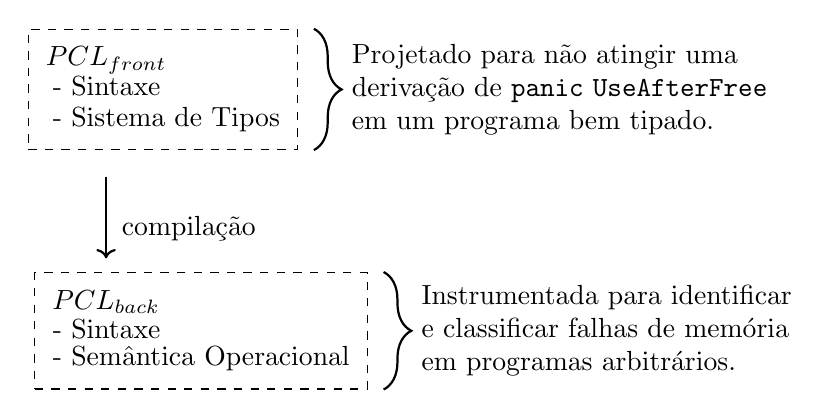
\begin{tikzpicture}[
		squarednode/.style={rectangle, draw=red!60, fill=red!5, very thick, minimum size=5mm},
	]
		%Nodes
		\node (front) {$PCL_{front}$};
		\node (sintaxf)[
			below=0.1em of front,
			align=left,
			anchor=west,
			xshift=-0.8cm
			]{- Sintaxe};
		\node (types) [
			below=1.3em of front,
			align=left,
			anchor=west,
			xshift=-0.8cm
		] {- Sistema de Tipos};

		\node (back) [below=2.5cm of front]{$PCL_{back}$};
		\node (sintaxb)[
			below=0.2em of back,
			align=left,
			anchor=west,
			xshift=-0.8cm
			]{- Sintaxe};
		\node (semantics) [
			below=1.3em of back,
			align=left,
			anchor=west,
			xshift=-0.8cm
		] {- Semântica Operacional};

		\node (boxfront) [draw, dashed, fit=(front) (sintaxf) (types), inner sep=0.1cm] {};

		\node (boxback) [draw, dashed, fit=(back) (sintaxb) (semantics), inner sep=0.1cm] {};
		
		%Lines
		\draw[->, thick, shorten >= 8pt] ($(front) + (0, -42pt)$) -- (back) node[midway, right=2pt] {compilação};

		\draw[decorate, decoration={brace, amplitude=10pt}, thick]
			($(boxfront.north east) + (2mm, 0)$) -- ($(boxfront.south east) + (2mm, 0)$) node[midway,right=10pt, align=left] 
			{
				Projetado para não atingir uma \\ 
				derivação de $\KW{panic}$ $\KW{UseAfterFree}$ \\ 
				em um programa bem tipado.
			};

		\draw[decorate, decoration={brace, amplitude=10pt}, thick]
			($(boxback.north east) + (2mm, 0)$) -- ($(boxback.south east) + (2mm, 0)$) node[midway,right=10pt, align=left] 
			{
				Instrumentada para identificar \\ e classificar falhas de memória \\ em programas arbitrários.
			};
	\end{tikzpicture}
	\vspace{0.3cm}
	\legend{Fonte: Os Autores.}
\end{figure*}



Este trabalho contribui para a discussão de falhas de memória e serve como um meio flexível de provar outras estratégias não convencionais em um campo mais neutro. Dessa forma, ele permite estratégias \emph{bottom-up} no desenvolvimento de linguagens, em que primeiro decide-se e prova-se uma estratégia de memória, para depois desenvolver a linguagem que a envolve.

%	1.4 Organização
\section{Organização}

O restante deste trabalho é organizado da seguinte forma: no Capítulo \ref{chap2} são elaborados conceitos básicos para o entendimento do projeto. Isso inclui uma explicação simples de semântica operacional e sistema de tipos, junto de uma elaboração sobre falhas de memória: significado, tipos e soluções propostas ao longo dos anos. No Capítulo \ref{chap3} é introduzido $PCL_{back}$, a linguagem-alvo de compilação do projeto. Para isso, elabora-se sobre as suas estruturas de avaliação, regras e correspondência com os erros do Capítulo~\ref{chap2}. Com esses dois capítulos, define-se a base do projeto. A partir desse ponto, passa-se a discorrer um caso de uso do sistema. O Capítulo \ref{chap4} discorre sobre os conceitos necessários para o desenvolvimento da linguagem $PCL_{front}$, explicada no Capítulo \ref{chap5}. O projeto é concluído pelo Capítulo \ref{chap7}.

% 1. Introdução
%	1.1 Motivação
%	1.2 Related Work
%	1.3 Objetivos
%	1.4 Organização
% 2. Background
\chapter{Background}

Este capítulo introduz alguns conceitos e definições essenciais ao projeto. 
Outros conceitos, específicos ao domínio do caso de uso da linguagem de front-end,
são elaborado no Capítulo \ref{chap4}. 

%	2.1 O que é Semantica Operacional
\section{Semântica Operacional}
\todo[inline]{Como \emph{definir} semântica operacional? Usar o livro do Nielson e do Slonneger }

\section{Julgamento de Tipos}
\todo[inline]{Como \emph{definir} julgamento de tipos? Usar o livro do Pierce }

%   2.2 Erros de memória
\section{Falhas de Memória}
\label{sec:mem-error}

\todo[inline]{Falar aqui de falhas, erro, fracasso, vindo do \emph{Basic Concepts and Taxonomy of Dependable and Secure Computing}} 

Basic Concepts and Taxonomy of Dependable and Secure Computing

% aqui fica especificamente se tratando de memória, mas revisar 
Falhas de memória ocorrem quando um acesso à memória consiste em comportamento
indefinido (UB). Essas falhas, ou no coloquial \emph{bugs}, podem ser ativas, 
gerando um Erro e movendo o programa para um estado incorreto; ou dormentes, 
existindo como possíveis vetores de ataque para agentes maliciosos capazes de 
ativar essa falha. 

As falhas de memória podem ser classificas em 5 classes: falha Espacial, 
Temporal, de Tipo, de Inicialização e de Condição de Corrida \cite{Apple22,Google24}.
\emph{Bugs} de memória podem ser subdivididos de mais formas \cite{7KINGDOMS,CWELIST},
tendo em conta falhas mais específicas ao domínio do programa. 
O uso das classes é mais interessante para o domínio deste projeto:
cada uma delas mapeia uma série de problemas para soluções específicas e disjuntas das demais. 
Ou seja, a solução para os problemas advindos de cada uma dessas classes pode ser 
pensada independentemente. 

% Memory safety bugs, as it concerns low level languages, can be subdivided in 5 classes: 
% Spacial, Temporal, Type, Initialization and Data-Race Safety. 
% Even though memory safety bugs can be subdivided in many more ways \cite{7KINGDOMS,CWELIST},
% each of those classes maps to a distinct mechanism for solving them. 
% Spacial safety can be solved with dependent types \cite{tarditi2018checked} and 
% runtime bounds checks\cite{CYCLONE1}; Temporal safety can be solved with 
% Garbage Collection (GC), memory regions\cite{REGMEM}, a static alias 
% analyzer\cite{Stjerna1684081}, key-lock systems \cite{FATPOINTERS, CCURED}, 
% and more. Both Type and Initialization can be solved by imposing stricter
% constraints on declarations and type conversions. Data-Race safety is beyond
% the scope of this project.
\todo[inline]{Anotar que os exemplos foram em parte retirados do site do \emph{CWE}}

\subsection{Falhas Espaciais}
\label{sec:mem-error:spacial}

Essa classe de falhas ocorre quando há manipulação de memória a uma região 
além do espaço alocado. Erros associados a acessos de memória em \emph{buffers} 
podem ser classificados amplamente como \emph{Out-of-Bounds-Read} ou \emph{Out-of-Bounds-Write} 
(leitura ou escrita fora dos limites). 
Podendo ocorrer na pilha ou na memória, para o final ou para o começo do \emph{buffer}, 
devido a um cálculo incorreto de tamanho do \emph{buffer} ou de índice de acesso. 
Fundamentalmente, esses erros são associados ao acesso arbitrário a memória e 
à falta de validação adequada.

Um exemplo dessa falha é um \emph{Buffer Under-Read}, 
leitura de um \emph{buffer} para uma posição anterior ao começo. No trecho a seguir
não se checa se $idx \ge 0$, possivelmente acessando memória antes do ponteiro.

\begin{lstlisting}[language=C ,label={lst:spacial-error-c}, caption=Exemplo de uma Falha Espacial]
int get_val(int* list, int len, int idx){
	if(idx < len) return list[idx];
	else return -1;
}
\end{lstlisting}

Falhas espaciais podem ser resolvidas de duas grandes formas. Há os tipos dependentes de Checked C \cite{CHECKEDC}, que verificam em tempo de compilação, usando informações de tipo, se um acesso está nos limites do buffer. Essa estratégia é menos comum, porém não adiciona nenhum impacto na performance do código. 
O método mais adotado atualmente é o de checagem de limite em tempo de execução. Nele, adiciona-se junto ao ponteiro a informação de tamanho do \emph{buffer} apontado, criando um \emph{fat-pointer} (ponteiro gordo). Assim, a cada acesso, verifica-se se este está dentro dos limites do \emph{buffer}, se não estiver, gera uma terminação controlada. Linguagens como Rust, Zig e Go se utilizam desse mecanismo, entretanto sob o nome de \emph{slices}.


\subsection{Falhas Temporais}
\label{sec:mem-error:temporal}

Essa classe de falhas ocorre quando há acesso a uma região de memória não mais ativa no momento. Ela engloba casos de \emph{Use-After-Free} e \emph{Use-After-Return}, assim como erros associados a função free de C. 
O caso de \emph{Use-After-Free}, é uma descrição de todo e qualquer acesso a \emph{heap} quando o objeto que se encontrava no local já havia sido liberado. Quando ocorre na pilha pode ser descrito pelo nome mais específico 
\emph{Return-of-Stack-Variable-Adress}, sendo o acesso a um endereço na pilha que já foi liberado pelo desempilhamento desta.

Um exemplo dessa falha é o seguinte \emph{Use-After-Free}. Nele, num caminho de erro do código, libera-se o ponteiro $ptr$. Entretanto no momento de logar esse erro, utiliza-se esse mesmo ponteiro liberado, gerando uma falha que pode escalar a erro dependendo do contexto de execução:
\begin{lstlisting}[language=C, label={lst:temporal-error-heap-c}, caption=Exemplo de uma Falha Temporal na \emph{Heap}]
char* ptr = (char*)malloc (SIZE);  
if (err) {
	abrt = 1;  
	free(ptr);
}  
...  
if (abrt) {
	logError("operation aborted before commit", ptr);
}
\end{lstlisting}

Outro exemplo, agora de \emph{Return-of-Stack-Variable-Adress}, retorna um \emph{buffer} alocado na pilha. Acesso a esse elemento pode reescrever a pilha de outras funções, sendo uma falha grave.

\begin{lstlisting}[language=C, label={lst:temporal-error-stack-c}, caption=Exemplo de uma Falha Temporal na Pilha]
char* getName() {
   char name[STR_MAX];  
   fillInName(name);  
   return name;
}
\end{lstlisting}

Fundamentalmente, a classe lida com leitura e escrita a regiões de memória não estáticas, ou seja, alocações na pilha, que são removidos no fim do escopo; e alocações na memória, que podem ser arbitrariamente de-alocados.


% Garbage Collection (GC)
\phantomsection
\label{sec:mem-error:GC}
A mitigação dessa classe de erros é a mais ampla e complexa desta lista. Desde a sua invenção em 1959\todo{citar}, uma das soluções mais completas presente tem sido o uso de um GC (coletor de lixo). Esse mecanismo detecta e retorna automaticamente memória alocada e não mais utilizada para o OS. Em troca, o programa sofre breves pausa periódicas (GC \emph{pauses}) na execução e a gerência do GC custa processamento que certos ambientes não tem disponível para gastar.

% Memory regions\cite{REGMEM}
\phantomsection
\label{sec:mem-error:MemReg}
Outra estratégia que emergiu do mundo de linguagens funcionais foi o de regiões de memória \cite{REGMEM}. Elas foram propostas como alternativa mais eficiente e previsível de gerência de memória que GC para MLKit. Nela, realiza-se as alocações em regiões, fazendo a gerência das regiões ao invés das alocações individuais. O projeto Cyclone trouxe esse conceito de regiões para lingaugens imperativas no começo do milenio \cite{CYCLONEMEM}, adicionado diversos mecânismos para adequar essa gerência para o novo meio.

%key-lock systems \cite{FATPOINTERS, CCURED},
\phantomsection
\label{sec:mem-error:KeyLock}
Um contemporâneo de Cyclone, CCured \cite{CCURED}, utilizou-se de um sistema de \emph{key-lock} para evitar falhas temporais. Nele, mantinha-se uma tabela global com uma chave para cada alocação. Realiza-se um verificação, na hora do acesso, se a chave ainda era válida, caso não fosse, havia uma terminação controlada. Esse método se demonstrou muito ineficiente. Mais recentemente, um projeto adicionou um sistema similar usando fat-pointers em Checked C \cite{FATPOINTERS}, mantendo esses metadados mais próximos dos dados reais e aumentando significativamente a performance.

%borrow checker
\phantomsection
\label{sec:mem-error:BorrowChecker}
Um metodo alternativo, com gerencia automática de memória é o borrow checker de Rust. Nele, limita-se o \emph{aliasing} de ponteiros e adiciona-se notações para que o acesso a memória possa ser validado em tempo de compilação. No Capítulo 4 \ref{chap4} será entrado em mais detalhes sobre esse sistema.

\subsubsection{Free}
\label{sec:mem-error:temporal:free}

\newcommand{\FREE}{\lstinline[language=C]|free()| }

Um componente importante dessa classe são as falhas associadas a liberação de memória, principalmente tratando-se da função \FREE da \emph{stdlib} de C. Falhas como \emph{Double-Free} (chamar \FREE para um endereço liberado), \emph{Free of Memory not on the Heap} (chamar \FREE em um ponteiro que não aponta para a \emph{heap}), \emph{Free of Pointer not at Start of Buffer} (chamar \FREE com um ponteiro que não inicia a lista) e \emph{Release of Invalid Pointer or Reference} (chamar uma função de liberação de memória para memória alocada com outro sistema) ocorrem devido a uma ação que corrompe a estrutura de dados usadas para gerir alocação. Assim, alocações subsequentes são UB e podem escalar a erros.

Um grande componente de soluções de memória temporal como o GC \ref{sec:mem-error:GC}, as Regiões de Memóriaz \ref{sec:mem-error:MemReg} e o \emph{Borrow Checker} \ref{sec:mem-error:BorrowChecker} é a dispensa da liberação manual de memória. Isso diminúi a superfície de falha do código, evitando possíveis erros.

\subsubsection{Nullptr}
\label{sec:mem-error:temporal:null}

Acessar o ponteiro nulo é um caso interessante nessa taxonomia de classes. Não pode-se dizer que essa ação é, firmemente, uma falha de inicialização \ref{sec:mem-error:init} ou uma falha temporal \ref{sec:mem-error:temporal}. Afinal, o valor nunca é liberado ou inicializado em função do tempo. Mesmo assim, escalar essa falha ao erro tende fazer o OS interromper o programa. Em certos sistemas, pode ser usado para realizar ataques mais severos \cite[p.4]{MemErrorPastPresentFuture}.

O ponteiro nulo é um elemento comum da maioria das linguagens, sendo elemento da linguagem mais influente da história. Entretanto, para lidar com referências é não necessário o seu uso. Linguagens funcionais, assim como inspiradas nelas - como Rust, se utilizam de tipos somatórios (\emph{tagged unions, variants, choice types, ...}) para representar a ausência de um valor, mantendo as referências não anuláveis.

A seção se encontra aqui, pois há a interação que passar o ponteiro nulo para a função \FREE gera uma falha \emph{Free of Memory not on the Heap}, visto que o endereço do nulo tende a ser 0, que não é um valor na \emph{heap} do programa.


\subsection{Falhas de Inicialização}
\label{sec:mem-error:init}

Essa classe de falhas ocorre quando há acesso a uma região de memória alocada, mas ainda não inicializada. Nesse caso, a leitura do espaço não inicializado gera valores incoerentes. No caso de ponteiros, pode-se acessar locais de memória arbitrários.

Erros de inicialização podem existir em contextos estáticos ou dinâmicos. No caso de variáveis, somatórios (\emph{tuples, structs, records, ...}) e lista de tamanho fixo, pode-se avaliar a inicialização do campo com uma análise estática de árvore. Para listas de tamanho dinâmico não há como realizar essa avaliação a tempo de compilação, por isso é de preferência que a API da linguagem requeira que a lista seja inicializada com valores base para os campos, evitando acessos a campos não inicializados. Isso também se estende as estruturas estáticas compostas, a inicialização e uso parcial delas pode gerar erros e dificulta a análise. Uma gerência mais restritiva, obrigar o programador a inicializar toda a estrutura não é um regime restritivo e incentiva boas práticas de código.

Um exemplo dessa falha é o acesso a \emph{string} em um caminho que não incializa ela, que vir ler valores arbitrários na \emph{heap}.

\begin{lstlisting}[language=C, label={lst:initialization}, caption=Exemplo de uma Falha de Inicalização com Strings]
char *test_string;
if (i != err_val){
	test_string = "Hello World!";
}
printf("%s", test_string);
\end{lstlisting}


\subsection{Falhas de Tipo}

Essa classe de erros ocorre quando há acesso a uma região de memória com o tipo incorreto. Ela ocorre no caso de cast incorretos de pointers tanto para tipos de tamanhos diferentes, como com layouts diferentes. Essa classe de erros é interessante pois é nela em que há a maior intersecção com \emph{undefined behavior}. UB é um tópico complicado e um buraco sem fundo que não será elaborado sobre. Mas, brevemente, o erro no caso do cast pode ser de ler a memória incorretamente, mas também pode ser por alguma otimização do compilador, que ou mudou o layout do objeto de origem/destino, ou alterou o resultado da operação pois a ação era UB.

\subsection{Falhas de Condição de Corrida}

Essa classe de falhas compreende todas os problemas gerados com código concorrente/paralelo. Essa classe é extremamente complexa e está fora do escopo deste projeto. Caso fique de curiosidade ao leitor, o livro \todo{Citar um livro} trata bem desse assunto. 

% 2. Background
%	2.1 O que é Semantica Operacional
%   2.2 Erros de memória
% 3. PCL back
\chapter{PCL-back}

% This work introduces $PCL_{back}$, a C-like core language de-
% signed to detect memory safety violations and to classify
% them. It is designed to be simple, for ease of developing
% proofs, but expressive enough to express common memory
% errors in C. Its syntax is defined as such:

Tendo em vista as falhas de memória descritas na seção \ref{sec:mem-error}, e visando analisá-las mais profundamente, é necessário desenvolver uma linguagem alvo para o fim de prova via compilação. A meta desse projeto é ter uma base relativamente agnóstica a solução a ser provada. Assim, introduz-se $PCL_{back}$, uma linguagem núcleo similar a C desenvolvida para detectar violações de segurança de memória e classificá-las. Ela é definida por sintaxe e semântica operacional \emph{small-step}. 

A escolha de C como base serviu para englobar todos as falhas de memórias, visto que C é uma linguagem que permite acesso e manipulação (quase) irrestrita à memória. Ou seja, pode-se expressar todas as falhas na seção \ref{sec:mem-error}. Essa é uma razão bem circular, as falhas são comuns em C porque este permite acesso brando a memória e assim elas são descritas; a linguagem que melhor reproduz elas é C, pois tem acesso \emph{laissez-faire} a memória.


%	3.1 Syntax
\section{Sintaxe}

A sintaxe baseada em C também se demonstrou familiar e facilitou a compreensão dos problemas e exemplos. Adicionalmente, esta é uma linguagem de expressões, permitindo certos padrões funcionais. Mesmo destoando de C, essa característica emergiu acidentalmente da implementação de funções na linguagem. A  sintaxe é definida em \ref{fig:pclback:sintax}.
\todo{Adicionar linebreak para fazer o split de das regras em várias páginas?}
\begin{figure*}[ht]
	\begingroup
	%\setlength{\jot}{-0.2ex} 
		\begin{align*}
			Locals \ni l ::&= l^m \OR l^p &&\\ 
			Value \ni v ::&= n \OR l && \\
			BinOp \ni op ::&= + | - | * | < | > | = | \land | \lor \\
			Expression \ni e ::&= x \OR v \\
			&\NLOR e\; op\; e \OR !e  \\
			&\NLOR \text{*}e \OR \&x \\
			&\NLOR e;e \; \OR \{\,e\,\} \; \\ 
			&\NLOR \mathbf{malloc}(e) \OR \mathbf{free}(e, e) \; \\ 
			&\NLOR \mathbf{let}\; x[n] \OR e := e \; \\
			&\NLOR \mathbf{if}(e) \; e \; \mathbf{else} \; e \; \OR \mathbf{while}(e) \; e \\
			&\NLOR f(\bar e) \\ 
			&\NLOR \mathbf{panic}\;pcode \\ 
			PanicCodes \ni pcode ::&= \mathbf{OutOfBoundsRead}\\
			&\NLOR \mathbf{OutOfBoundsWrite}\\
			&\NLOR \mathbf{NullPtrDereference}\\
			&\NLOR \mathbf{UserError}\\
			&\NLOR \mathbf{UseAfterFree}\\
			&\NLOR \mathbf{UninitializedAcess}\\
			&\NLOR \mathbf{FreeMemoryNotOnHeap}\\
			&\NLOR \mathbf{PartialFree}\\
			&\NLOR \mathbf{DoubleFree}\\
			Function \ni F ::&= \mathbf{let} \; f(\overline{x})\; e \; F \; | \; \mathbf{let}\;() \; e \\
			Globals \ni G ::&= \mathbf{global}\; x[n] \;G \;|\; F
		\end{align*}
	\endgroup
	\caption{Sintaxe de $PCL_{back}$}
	\label{fig:pclback:sintax}
\end{figure*}
% NOTE: funciona, yeyyyyyy
\FloatBarrier

Nela, o termo $x$ cobre todos os possíveis nomes de variáveis em um programa. 
$f$ cobre todos os nomes de funções. O conjunto $PanicCodes$ são so tipos de falhas de memória, que podem ser divididos nas 5 classes (mais extras) da seguinte forma:
\begin{enumerate}
	\item $\mathbf{OutofBoundsRead}$ e $\mathbf{OutofBoundsWrite}$ são falhas espaciais (\ref{sec:mem-error:spacial}), sendo leitura e escrita para além dos limites do \emph{buffer} respectivamente.
	\item $\mathbf{UseAfterFree}$, $\mathbf{FreeMemoryNotOnHeap}$, $\mathbf{Partial ree}$ e $\mathbf{Double Free}$ são falhas temporais (\ref{sec:mem-error:temporal}), sendo uso de uma região liberada de memória para o primeiro e corrupção da estrutura alocadora por diversos meios para os demais.
	\item $\mathbf{UninitializedAccess}$ é uma falha de inicialização (\ref{sec:mem-error:init}), sendo o acesso ao valor alocado, mas não inicializado. 
	\item $\mathbf{NullPtrDereference}$ é uma falha específica ao domínio de C, em que essa linguagem se baseia (\ref{sec:mem-error:temporal:null}), sendo o acesso ao ponteiro nulo.
	\item $\mathbf{UserError}$ é uma interrupção manual de usuário, similar a \lstinline[language=C]|exit(1)| em C. É usado como mecanismo de emissão de erros controlados que terminam a execução.
\end{enumerate}

\noindent Acima há a omissão das falhas de tipos, pois $PCL_{back}$ não é tipado. Os seus valores, locais $l$ e números $n$, encaixam, independente do tamanho, em uma célula. Há também omissão das falhas de condição de corrida. Elas não são representáveis nessa linguagem, pois não possui mecanismos de paralelização.

Esses códigos de pânico $pcode$ servem como interrupções na avaliação da linguagem, indicando uma falha de memória. Eles são um importante componente no processo de compilação e prova. Um método de segurança de memória não precisa ser compreensivo e cobrir todas as falhas geradas, mas se a sua compilação para $PCL_{back}$ não gerar o conjunto de $PanicCodes$ que se almeja evitar, então afirma-se que o método é correto no que se propõem. Ou seja, dado um processo de indução estrutural em um $PCL_{back}$ compilado de uma linguagem que deseja evitar falhas espaciais, basta que na derivação nunca se atinjam as expressões $\KW{panic}\;\KW{OutofBoundsRead}$ e $\KW{panic}\;\mathbf{OutofBoundsWrite}$.

%	3.2 Memory Model
\section{Modelo de Memória}

O layout de memória de um programa em C tem vários componentes\todo{Adicionar citação e um diagrama. Provavelmente retirar do livro de C}: o segmento de texto, que contém o programa em si; a seção de dados, que guarda elementos globais, assim como \emph{strings} literais e outros elementos escritos no código; a pilha e a \emph{heap}. A pilha é o lugar em que variáveis locais são alocadas e chamadas de funções são geridas. Ela realiza alocações de tamanho conhecido em tempo de compilação e libera essa memória no final do escopo da variável associada. A \emph{heap} é o lugar em que alocações dinâmicas são colocadas, seja porque o tamanho ou a duração não são conhecidos em tempo de compilação.

A dinâmica entre alocações manuais, aquelas que acontecem na \emph{heap}, e alocações estáticas, aquelas que acontecem na pilha, é um componente importante na reprodução de \emph{bugs} de memória. Falhas na \emph{heap} tendem a ser mais difíceis de encontrar e lidar, pois o processo de requisitar memória e liberá-la manualmente tende a aumentar a superfície de falhas. 

Com o intuito de modelar essa dinâmica, a memória em $PCL_{back}$ usa dois ambientes disjuntos, $p$ para modelar a pilha e $m$ para modelar a \emph{heap}, que, com o intuito de diminuir os estrangeirismos, poderá ser referida como memória a partir deste ponto. 

\subsection{Ponteiros}
\label{sec:pcl-back:ptr}

Com essa distinção, pode-se notar que o elemento da sintaxe responsável por indexar a memória, a localização $l$, é divida em $l^p$ e $l^m$. Nesse contexto, $p$ e $m$ são etiquetas de $l$ que indicam se essa localização é para a pilha ou para memória. Essas localizações também possuem outros metadados, utilizados na avaliação da linguagem para detectar as falhas. Assim, a representação interna dos locais pode ser escrita como:
\begin{figure*}[ht]
	\begin{align*}
		l^p\{i, k, o, s \} && l^m\{i, k, o, s \}
	\end{align*}
	\caption{Layout dos metadados dos locais.}
	\label{fig:ptr:metada}
\end{figure*}
\todo{Fazer um diagrama mais legal?}

Nela, $i$ é o índice de acesso à memória; $k$ é a uma chave única, gerada através da função $\mathbf{newkey}$, que serve para validar os acessos quanto a falhas temporais; $o$ é o \emph{offset} (desvio) do índice base $i$, que recebe o valor das somas e subtrações, ao invés de alterar o índice diretamente; e $s$ é o tamanho da região alocada na memória, que serve para validar os acessos quanto a falhas espaciais. Esses metadados não são acessíveis na escrita do código, mas na semântica operacional tem seus valores internos expostos à avaliação usando a anotação de chaves acima.

\subsection{Pilha}

A pilha é uma lista de elementos, que podem ser valores $v \in \{l, n, \bot, -\}$ ou códigos de controle $c_{ctrl} \in \{\mathbf{stack},\mathbf{func}\}$. Dentre os valores, $l$ e $n$ são os elementos de locais e números da sintaxe da linguagem. $\bot$ e $-$, assim como em \citet{WESSEL2019}, são elementos utilizados na representação da inicialização de um valor, representando um espaço alocado, mas ainda não inicializado, e um espaço não alocado, respectivamente. 

Junto desses elementos guarda-se uma fechadura $k \in \mathbb{N}\text{*}$. Esse elemento serve para a checagem de falhas temporais, similar ao sistema de \emph{key-lock} \ref{sec:mem-error:KeyLock}. Para um acesso ser válido, é necessário que a chave $k$ do local $l$ que tenta acessar a célula seja igual à fechadura $k'$ salva junto ao valor na célula. Valor de controle, junto do $\bot$ e $-$ sempre são empilhados com a chave de valor 0 associada. Uma pilha $p$ da linguagem pode ser definida como uma lista de pares, com o primeiro elemento sendo ou um valor, ou um código de controle, e com o segundo elemento sendo a fechadura de acesso, tal como $p := [(v\,|\,c_{ctrl}, k)]$.

Os códigos de controle citados existem para essa lista se comportar como um pilha de um sistema. Quando se inicia um escopo, coloca-se no fim da lista um código de controle. Chegando no final desse escopo, removem-se elementos do final da lista até atingir o código escolhido, emulando a impermanência dos elementos de uma pilha. Na semântica, utiliza-se das funções $\mathbf{pop}_{stack}(p)$ e $\mathbf{pop}_{func}(p)$ para descrever a ação de remover os elementos da lista até o código de controle $\mathbf{stack}$ ou $\mathbf{func}$. Elas são definidas da seguinte forma:

\begin{figure}[ht]
	\begin{align}
		&\mathbf{pop}_{stack}(p) = \mathbf{pop}(p, stack) \label{fig:def:pop1}\\
		&\mathbf{pop}_{func}(p) = \mathbf{pop}(p, func) \label{fig:def:pop2}\\
		&\mathbf{pop}((v, \_) : t, c_{ctrl}) = \mathbf{if} \; v \neq c_{ctrl} \;\mathbf{then} \; \mathbf{pop}(t, c_{ctrl}) \; \mathbf{else} \; t  \label{fig:def:pop3}\\
		&\mathbf{pop}([], c_{ctrl}) =  [] \label{fig:def:pop4}
	\end{align}
	\caption{Função que define a operação $\mathbf{pop}$}
	\label{fig:def:pop}
\end{figure}

A notação para descrever as funções neste projeto é similar a Haskell \cite{HASKELL}, com casamento de padrões nos argumentos das funções e as definições recursivas. Para o caso acima, em \ref{fig:def:pop1} e \ref{fig:def:pop2} definem as funções $\mathbf{pop}_{stack}(p)$ e $\mathbf{pop}_{func}(p)$ com base na função $\mathbf{pop}(p, v)$, usando como valor inicial de $v$ os seus elementos subscritos. Em \ref{fig:def:pop3} e \ref{fig:def:pop4} realiza a lógica. Se os argumentos casarem o padrão $h : t$, que nesse contexto é a lista poder ser dividida entre o elemento no fim $(v, \_)$ e no restante $t$, então executa-se \ref{fig:def:pop3}. Se a lista for vazia, representada por $[]$, realiza-se \ref{fig:def:pop4}. $(v,\_)$ também é um casamento de padrão, que atribui o nome $v$ para o primeiro elemento da dupla, o valor, e descarta o segundo, a chave. Com esses elementos, \ref{fig:def:pop3} checa se o valor no fim da lista é igual ao código de controle $c_{ctrl}$, se é retorna o restante da lista $t$, se não chama $\mathbf{pop}(t, c_{ctr})$ recursivamente para o restante da lista. Isso descarta elementos do topo da lista até finalmente descartar o $c_{ctrl}$ ou, pela definição \ref{fig:def:pop4}, chegar no final e retorna a lista vazia.

Outras funções similares existem para descrever o acesso, inserção de elementos e edição de elementos na pilha. A inserção no topo da pilha, tal qual em Haskell, utiliza-se o símbolo $:$ como uma operação binária de valor e pilha para pilha. Escreve-se $v : p$ para realizar o empilhamento de $v$ em $p$, retornando $p'$ com $v$ no topo. Caso se deseje empilhar várias cópias de um elemento na pilha, subscreve-se este com um número indicando a quantidade. Dessa forma, escrever $\bot_n : p$ empilha $n$ vezes o valor $\bot$ no topo da pilha. 

O acesso a pilha $p$ na posição $i$, $p(i)$ é descrito pela função:

\begin{figure}[ht]
	\begin{align}
	&p(i) = \mathbf{get}(i, \mathbf{top}(p) - 1, p) \label{fig:def:px1}\\
	&\mathbf{get}(i, size, p_v : p_r) = \mathbf{if}\;i = size \;\mathbf{then}\;p_v\;\mathbf{else}\;\mathbf{get}(i, size - 1, p_r) \label{fig:def:px2}\\
	&\mathbf{get}(\_, \_, []) = (-,0) \label{fig:def:px3}
	\end{align}
	\caption{Função que define a operação de acesso $p(i)$.}
	\label{fig:def:px}
\end{figure}

A notação é similar a \ref{fig:def:pop}, usando a primeira expressão, \ref{fig:def:px1}, para chamar uma função auxiliar associada, neste caso $\mathbf{get(i, size, p)}$ com o índice de acesso $i$, o tamanho atual da pilha $size$ e a pilha $p$ em sí. \ref{fig:def:px1} checa se o índice é igual ao tamanho $size$, se sim retorna o fim da lista, ou seja, o topo da pilha, se não repete recursivamente para o restante da lista, com o $size - 1$. Isso se repete até $i = size$ ou, em \ref{fig:def:px3}, chegar no fim da pilha, retornando $(-,0)$, que representa o valor não inicializado.

A função auxiliar $\mathbf{top}(p)$ utilizada em \ref{fig:def:px1} retorna o tamanho da lista. Esse tamanho também pode ser interpretado como índice para o elemento acima do último elemento da lista. Esse fato é usado na notação da semântica operacional para gerar o índice das alocações na pilha \todo{Referir-se a regra let.}. Uma definição com a notação atual pode ser escrita como:

\begin{figure}[ht]
	\begin{align}
	&\mathbf{top}(\_ : t) = 1 + \mathbf{top}(t) \label{fig:def:top1}\\
	&\mathbf{top}([]) = 0 \label{fig:def:top2}
	\end{align}
	\caption{Função que calcula o tamanho da pilha $p$.}
	\label{fig:def:top}
\end{figure}

Essa é a definição clássica de calcular o tamanho de uma lista recursivamente. Adicionando 1 ao resultado até o final da lista, que retorna 0 para a conta.

Para inserir um valor $v$ na posição $i$ da pilha $p$, escreve-se $p[i \mapsto v]$. Essa operação retorna uma nova pilha $p'$ com o valor atualizado na posição. Ela é melhor visualizada como a operação de indexação e atribuição a um \emph{buffer} em C, da forma \lstinline[language=C]|p[i] = v|. Mas ao quesito de rigorosidade, também se define no estilo funcional da seguinte forma:

\begin{figure}[ht]
	\begin{align}
	&p[i \mapsto v] = \mathbf{set}(i, \mathbf{top}(p) - 1, v) \label{fig:def:set1}\\
	&\mathbf{set}(i, size, (v_p, k_p) : p_r) = \mathbf{if}\;i = size \;\mathbf{then} \nonumber\\ 
	&\quad\quad(v, k_p) : p_r\;\mathbf{else}\;(v_p, k_p) : \mathbf{set}(i, size - 1, p_r) \label{fig:def:set2}\\
	&\mathbf{get}(\_, \_, []) = [] \label{fig:def:set3}
	\end{align}
	\caption{Função que insere o valor $v$ na posição $i$ da pilha $p$.}
	\label{fig:def:set}
\end{figure}

Ela usa a notação de empilhamento ($:$) com toda a sua expressividade. Após em \ref{fig:def:set1} definir via uma função auxiliar a operação, \ref{fig:def:set2} checa se $i = size$, se for troca o topo da lista atual para uma dupla com a chave anterior e o novo valor. Se $i \neq size$, concatena o topo atual da pilha com o restante da operação. Isso resulta em uma pilha nova final $p'$ cujo único elemento diferente é o da posição de índice $i$. Caso o índice seja para fora da pilha, eventualmente \ref{fig:def:set3} será atingido, terminando a execução e retornando a pilha inalterada.

Uma notação alternativa, para quando se precisa alterar várias posições na pilha para um mesmo valor é $p[i_{m..n} \mapsto v]$. Similarmente a empilhar vários elementos do mesmo valor, essa definição altera os valores da posição $i + m$ até a posição $i + n - 1$ para o valor $v$.


\subsection{\emph{Heap}}

A memória (\emph{heap}) é extremamente similar a pilha, porém sem os códigos de controle. Partindo disso, a memória $m$ é uma lista de pares, valor $v \in \{n, l, \bot, -\}$ fechadura $k \in \mathbb{N}$, podendo ser escrito na forma $m := [(v, k)]$. Essa lista pode ser imaginada infinitamente grande, tendo todas as células inicializadas com o valor $-$.

As células da memória são manualmente liberadas com a função $\mathbf{free}$ e alocadas com a função $\mathbf{malloc}$. Essa última usa uma função auxiliar $mathbf{loc(m,n)}$ para encontrar na memória $m$, $n$ células contíguas não alocadas (com o valor $-$) e retorna o índice do começo dessa região. Ela é descrita mais formalmente da seguinte forma:

\begin{figure}[ht]
	\begin{align}
	&\mathbf{loc}(m,n) = \mathbf{loc}'(m, n, 0, 1) \label{fig:def:loc1}\\
	& \mathbf{loc}'(m, n_0 , n_1, i) = \mathbf{if}\; m(i + n_1) \neq (-,0) \; \mathbf{then}\nonumber \\
	&\quad\mathbf{loc}'(m, n_0, 0, i + n_1 + 1)\; \mathbf{else} \nonumber\\
	&\quad\quad(\mathbf{if}\; n_0 = n_1 \; \mathbf{then}\; i \;\mathbf{else}\; \mathbf{loc}'(m, n_0, n_1 + 1, i)) \label{fig:def:loc2}
	\end{align}
	\caption{Função encontra em $m$, $n$ contíguas células não alocadas.}
	\label{fig:def:loc}
\end{figure}

\noindent Ela primeiro chama uma função auxiliar em \ref{fig:def:loc1}, com 0 para $n_1$, o tamanho atual da região encontrada,  e 1 para $i$, o índice de início de busca. Parte-se do índice de número um, mesmo a indexação da lista iniciando no 0, pois se reserva esse espaço para a implementação do ponteiro nulo. Em \ref{fig:def:loc2} realiza-se a computação: se o valor no índice $i$ da memória $m$ mais o tamanho da região atual encontrada $n_1$ não for o par $(-,0)$ (célula não alocada), então reinicia a busca, partindo no índice seguinte ao analisado nesse teste; se não for o caso, verifica-se se já se encontrou a região do tamanho esperado, se sim, retorna o índice $i$, que é o índice do começo desta, se não, avalia-se a célula seguinte, chamando $\mathbf{loc}'$ recursivamente, incrementando o valor da região encontrada em 1.

Na definição dessa função, utilizou-se a expressão $m(i)$ para indicar o acesso ao elemento de índice $i$ da memória $m$. Assim como o acesso na pilha, essa operação pode ser vista como uma simples indexação a um \emph{buffer}. Neste caso, como há a intuição da memória ser infinita, para qualquer índice $i$ há uma célula correspondente na memória. Como todas elas iniciam com o valor $(-,0)$, o comportamento de acessar para além do espaço alocado é o mesmo de quando isso acontece na pilha. A atribuição segue o mesmo padrão, inserir o valor $v$ no índice $i$ da memória $m$ é escrito como $m[i \mapsto v]$. Aqui omiti-se a definição porque estas são (quase) idênticas às definições da pilha, visto que a memória não pode ser realmente infinita. O mesmo segue para a atribuição de várias células com a notação $m[i_{m..n} \mapsto v]$ cujo comportamento é o mesmo que na pilha, porém no contexto da memória essa função é mais usada, visto que é  instrumental as definições de $\mathbf{malloc}$ e $\mathbf{free}$.


%	3.3 Operational Semantics
\section{Semântica Operacional}

% The language is defined by means of structural operational semantics, 
% which specifies a one-step relation between configurations (states). 
% One writes $F \vdash \St{e, a, p, m} \to \St{e', a', p', m'}$ to describe 
% the transition of state $\St{e, a, p, m}$ towards state $\St{e', a', p', m'}$ 
% under a global function definition environment $F$. 
% Within the state, $e$ is the program, $a$ is the names environment, 
% $p$ is the stack and $m$ is the heap. 

subdivido em 3 transições para avaliar um programa P
\ignoreLtex{
\infrule
    {\St{P, \{\}, []} \to_G^* \St{F_0, g, p}\quad\St{F_0, \{\}} \to_F^* \St{\mathbf{let}\;()\;e , F}}
    {F \vdash \St{\{e\}, ([],g),p,[]} \to^* \St{v, ([],g), p, m}} 
}

\subsection{Globais}

\ignoreLtex{
\infrule[Globals-collect]
    {\mathbf{newkey}() = k \quad \mathbf{top}(p) = i}
    {\St{\mathbf{global} \; x[n]\; G , g, p} \to_G\\ \St{G, g[x \mapsto l^p \{i, k, 0, n\}],(\bot, k)_n : p,}} 
}

\subsection{Funções}

\ignoreLtex{
\infrule[LetFunction-collect]
    {}
    {\St{\mathbf{let} \; f(\overline{x_i})\; e \; F_0 ,F} \to_F \St{F_0, F[f \mapsto \St{[\overline{x_i}], e}]}}
}

\subsection{Expressões}


\todo[inline]{Dar uma formatada mais legal nessas regras que esta meio feio}

\ignoreLtex{
\infrule[Compose-s]
    {F \vdash \St{e_1,a, p, m} \to \St{e_1',a', p', m'}}
    {F \vdash \St{e_1;e_2,a, p, m} \to \St{e_1';e_2,a', p', m'}}

\infrule[Compose]
    {}
    {F \vdash \St{v;e, a, p, m} \to \St{e, a, p, m}}
\infrule[Escopo]
    {}
    {F \vdash \St{\{e\},(a,g), p, m} \to \\ \St{\mathbf{pop}\; e,(\{\} : a, g),stack : p, m}}
\infrule[Pop-s]
    {F \vdash \St{e,a, p, m} \to \St{e',a', p', m'}}
    {F \vdash \St{\mathbf{pop}\;e,a, p, m} \to \St{\mathbf{pop}\;e',a', p', m'}} 
 \infrule[Pop]
    {\mathbf{pop}_{stack}(p) = p'}
    {F \vdash \St{\mathbf{pop}\;v,(frame : a, g), p, m} \to\\\St{v,(a, g), p', m}}

\infrule[Let]
    {\mathbf{top}(p) = i \andalso \mathbf{newkey}() = k \andalso l = l^p\{i, k, 0, n\}}
    {F \vdash \St{\mathbf{let}\; x[n],(fr : a, g), p, m} \to\\ \St{l, (fr[x \mapsto l] : a, g),(\bot, k)_n : p, m}} 

\infrule[Atribui-deref-ls]
    {F \vdash \St{e_1,a, p, m} \to \St{e_1', a', p', m'}}
    {F \vdash \St{\text{*}e_1 := e_2, a, p, m} \to \St{\text{*}e_1' := e_2, a', p', m'}} 

\infrule[Atribui-var-rs]
    {F \vdash \St{e, a, p, m} \to \St{e', a', p', m'}}
    {F \vdash \St{x := e, a, p, m} \to \St{x := e', a', p', m'}} 

\infrule[Atribui-deref-rs]
    {F \vdash \St{e,a, p, m} \to \St{e', a', p', m'}}
    {F \vdash \St{\text{*}l := e, a, p, m} \to \St{\text{*}l := e', a', p', m'}} 

\infrule[Atribui-var-obe]
    {a(x) = l^p\{i, k, o, s\} \andalso 0 > o \ge s}
    {F \vdash \St{x := v, a, p, m} \to \\ \St{\mathbf{panic}\;\mathbf{OutOfBoundsWrite}, a, p, m}}
    
\infrule[Atribui-var-uaf]
    {a(x) = l^p\{i, k, o, s\} \\ 0 \leq o < s\andalso p(i + o) = (v_p, k_p) \andalso k \neq k_p }
    {F \vdash \St{x := v, a, p, m} \to \\ \St{\mathbf{panic}\;\mathbf{UseAfterFree}, a, p, m}}

\infrule[Atribui-var]
    {a(x) = l^p\{i, k, o, s\} \\ 0 \leq o < s\quad p(i + o) = (v_p, k_p) \quad k = k_p }
    {F \vdash \St{x := v, a, p, m} \to \St{v, a, p[i + o \mapsto v], m}} 

\infrule[Atribui-deref-pilha-obe]
    {0 > o \ge s}
    {F\vdash\St{\text{*}l^p\{i, k, o, s\} := v, a, p, m} \to \\ \St{\mathbf{panic}\;\mathbf{OutOfBoundsWrite}, a, p, m}} 

\infrule[Atribui-deref-pilha-uaf]
    {0 \leq o < s\quad p(i + o) = (v_p, k_p) \quad k \neq k_p }
    {F\vdash\St{\text{*}l^p\{i, k, o, s\} := v, a, p, m} \to\\ \St{\mathbf{panic}\;\mathbf{UseAfterFree}, a, p, m}} 
    
\infrule[Atribui-deref-pilha]
    {0 \leq o < s\quad p(i + o) = (v_p, k_p) \quad k = k_p }
    {F\vdash\St{\text{*}l^p\{i, k, o, s\} := v, a, p, m} \to\\ \St{v, a, p[i + o \mapsto v], m}} 

\infrule[Atribui-deref-mem-npd]
    {i = 0}
    {F\vdash\St{\text{*}l^m\{i, k, o, s\} := v, a, p, m} \to\\ \St{\mathbf{panic}\;\mathbf{NullPtrDeref}, a, p, m}} 

\infrule[Atribui-deref-mem-obe]
    {i \neq 0 \quad 0 > o \ge s}
    {F\vdash\St{\text{*}l^m\{i, k, o, s\} := v, a, p, m} \to\\ \St{\mathbf{panic}\;\mathbf{OutOfBoundsWrite}, a, p, m}} 

\infrule[Atribui-deref-mem-uaf]
    {i \neq 0 \quad 0 \leq o < s\quad m(i + o) = (v_m, k_m) \quad k \neq k_m }
    {F\vdash\St{\text{*}l^m\{i, k, o, s\} := v, a, p, m} \to\\ \St{\mathbf{panic}\;\mathbf{UseAfterFree}, a, p, m}} 
    
\infrule[Atribui-deref-mem]
    {i \neq 0 \quad 0 \leq o < s\quad m(i + o) = (v_m, k_m) \quad k = k_m }
    {F\vdash\St{\text{*}l^m\{i, k, o, s\} := v, a, p, m} \to \\\St{v, a, p, m[i + o \mapsto v]}}

\infrule[Malloc-s]
    {F\vdash\St{e, a, p, m} \to\St{e', a', p', m'}}
    {F\vdash\St{\mathbf{malloc}(e),a, p, m} \to\St{\mathbf{malloc}(e'),a', p', m'}}
    
\infrule[Malloc]
    {\mathbf{loc}(m, n) = i \quad \mathbf{newkey}() = k \quad l = l^m\{i, k, 0, n\}}
    {F\vdash\St{\mathbf{malloc}(n),a, p, m} \to\St{l, a, p, m[i_{0..n} \mapsto (\bot,k)]}} 
    
\infrule[Free-ls]
    {F\vdash\St{e_1, a, p, m} \to\St{e_1', a', p', m'}}
    {F\vdash\St{\mathbf{free}(e_1, e_2),a, p, m} \to\St{\mathbf{free}(e_1', e_2),a', p', m'}}
    
\infrule[Free-rs]
    {F\vdash\St{e, a, p, m} \to\St{e', a', p', m'}}
    {F\vdash\St{\mathbf{free}(l, e),a, p, m} \to\St{\mathbf{free}(l, e'),a', p', m'}} 

\infrule[Free-mnh]
    {}
    {F\vdash\St{\mathbf{free}(l^p, n),a, p, m} \to\\ \St{\mathbf{panic}\;\mathbf{FreeMemoryNotOnHeap},a, p, m}}

\infrule[Free-memory-null] 
    {i = 0}
    {F\vdash\St{\mathbf{free}(l^m\{i, k, o, s\}, n),a, p, m} \to\\ \St{\mathbf{panic}\;\mathbf{FreeMemoryNotOnHeap},a, p, m}}
    
\infrule[Free-pf] 
    {i \neq 0 \quad o \neq 0 \lor s \neq n}
    {F\vdash\St{\mathbf{free}(l^m\{i, k, o, s\}, n),a, p, m} \to\\ \St{\mathbf{panic}\;\mathbf{PartialFree},a, p, m}}
    
\infrule[Free-df]
    {i \neq 0 \quad o = 0 \quad s = n \quad m(i) = (v_m, k_m) \quad k \neq k_m}
    {F\vdash\St{\mathbf{free}(l^m\{i, k, o, s\}, n),a, p, m} \to\\ \St{\mathbf{panic}\;\mathbf{DoubleFree},a, p, m}}

\infrule[Free]
    {i \neq 0 \quad o = 0 \quad s = n \quad m(i) = (v_m, k_m) \quad k = k_m}
    {F\vdash\St{\mathbf{free}(l^m\{i, k, o, s\}, n),a, p, m} \to\St{n,a, p, m[i_{0..n} \mapsto (-,0)]}}

\infrule[BinOp-ls]
    {F \vdash \St{e_1,a, p, m} \to \St{e_1', a', p', m'}}
    {F \vdash \St{e_1 \;op\; e_2, a, p, m} \to \St{e_1' \;op\; e_2, a', p', m'}} 

\infrule[BinOp-rs]
    {F \vdash \St{e,a, p, m} \to \St{e', a', p', m'}}
    {F \vdash \St{v \;op\; e, a, p, m} \to \St{v \;op\; e', a', p', m'}}

\infrule[BinOp]
    {\mathbf{binop}(op, v_1, v_2) = v'}
    {F \vdash \St{v_1 \;op\; v_2, a, p, m} \to \St{v', a, p, m}}

\infrule[Not-s]
    {F \vdash \St{e,a, p, m} \to \St{e', a', p', m'}}
    {F \vdash \St{!e, a, p, m} \to \St{!e', a', p', m'}}

\infrule[Not]
    {\mathbf{not}(v) = n}
    {F \vdash \St{!v, a, p, m} \to \St{n, a, p, m}}

\infrule[Var-obr]
    {a(x) = l^p\{i, k, o, s\} \quad 0 > o \ge s}
    {F \vdash \St{x, a, p, m} \to\\ \St{\mathbf{panic}\;\mathbf{OutOfBoundsRead}, a, p, m}}
    
\infrule[Var-uaf]
    {a(x) = l^p\{i, k, o, s\} \\ 0 \leq o < s\quad p(i + o) = (v_p, k_p) \quad k \neq k_p}
    {F \vdash \St{x, a, p, m} \to \St{\mathbf{panic}\;\mathbf{UseAfterFree}, a, p, m}}

\infrule[Var-ua]
    {a(x) = l^p\{i, k, o, s\} \\ 0 \leq o < s\quad p(i + o) = (v_p, k_p) \quad k = k_p \quad v_p = \bot}
    {F \vdash \St{x, a, p, m} \to \\ \St{\mathbf{panic}\;\mathbf{UninitializedAcess}, a, p, m}} 

\infrule[Var]
    {a(x) = l^p\{i, k, o, s\} \\ 0 \leq o < s\quad p(i + o) = (v_p, k_p) \quad k = k_p \quad v_p \neq \bot}
    {F \vdash \St{x, a, p, m} \to \St{v_p, a, p, m}}

\infrule[Ref]
    {a(x) = l^p}
    {F \vdash \St{\&x, a, p, m} \to \St{l^p, a, p, m}}
    
\infrule[Deref-s]
	{F \vdash \St{e,a, p, m} \to \St{e', a', p', m'}}
	{F \vdash \St{\text{*}e, a, p, m} \to \St{\text{*}e', a', p', m'}} 

\infrule[Deref-pilha-obr]
    {0 > o \ge s}
    {F \vdash \St{\text{*}l^p\{i, k, o, s\}, a, p, m} \to \\ \St{\mathbf{panic}\;\mathbf{OutOfBoundsRead}, a, p, m}}
    
\infrule[Deref-pilha-uaf]
    {0 \leq o < s\quad p(i + o) = (v_p, k_p) \quad k \neq k_p}
    {F \vdash \St{\text{*}l^p\{i, k, o, s\}, a, p, m} \to\\ \St{\mathbf{panic}\;\mathbf{UseAfterFree}, a, p, m}} 

\infrule[Deref-pilha-ua]
    {0 \leq o < s\quad p(i + o) = (v_p, k_p) \quad k = k_p \quad v_p = \bot}
    {F \vdash \St{\text{*}l^p\{i, k, o, s\}, a, p, m} \to\\ \St{\mathbf{panic}\;\mathbf{UninitializedAcess}, a, p, m}}

\infrule[Deref-pilha]
    {0 \leq o < s\quad p(i + o) = (v_p, k_p) \quad k = k_p \quad v_p \neq \bot}
    {F \vdash \St{\text{*}l^p\{i, k, o, s\}, a, p, m} \to \St{v_p, a, p, m}}

\infrule[Deref-memória-null]
    {i = 0}
    {F \vdash \St{\text{*}l^m\{i, k, o, s\}, a, p, m} \to\\ \St{\mathbf{panic}\;\mathbf{NullPtrDeref}, a, p, m}}

\infrule[Deref-memória-obr]
    {i \neq 0 \quad 0 > o \ge s}
    {F \vdash \St{\text{*}l^m\{i, k, o, s\}, a, p, m} \to\\ \St{\mathbf{panic}\;\mathbf{OutOfBoundsRead}, a, p, m}}
    
\infrule[Deref-memória-uaf]
    {i \neq 0 \quad 0 \leq o < s\quad m(i + o) = (v_m, k_m) \quad k \neq k_m}
    {F \vdash \St{\text{*}l^m\{i, k, o, s\}, a, p, m} \to\\ \St{\mathbf{panic}\;\mathbf{UseAfterFree}, a, p, m}}

\infrule[Deref-memória-ua]
    {i \neq 0 \quad 0 \leq o < s\quad m(i + o) = (v_m, k_m) \quad k = k_m \quad v_m = \bot}
    {F \vdash \St{\text{*}l^m\{i, k, o, s\}, a, p, m} \to\\ \St{\mathbf{panic}\;\mathbf{UninitializedAcess}, a, p, m}} 
    
\infrule[Deref-memória]
    {i \neq 0 \quad 0 \leq o < s\quad m(i + o) = (v_m, k_m) \quad k = k_m \quad v_m \neq \bot}
    {F \vdash \St{\text{*}l^m\{i, k, o, s\}, a, p, m} \to \St{v_m, a, p, m}}

\infrule[If-s]
    {F \vdash \St{e_1,a, p, m} \to \St{e_1', a', p', m'}}
    {F \vdash \St{\mathbf{if}\;(e_1)\; e_2\; \mathbf{else}\; e_3 ,a, p, m} \to\\ \St{\mathbf{if}\;(e_1')\; e_2\; \mathbf{else}\; e_3 ,a', p', m'}}
    
\infrule[If-true]
    {\mathcal{N}(v) \neq 0}
    {F \vdash \St{\mathbf{if}\;(v)\; e_1\; \mathbf{else}\; e_2 ,a, p, m} \to \St{e_1, a, p, m}} 
\infrule[If-false]
    {\mathcal{N}(v) = 0}
    {F \vdash \St{\mathbf{if}\;(v)\; e_1\; \mathbf{else}\; e_2 ,a, p, m} \to \St{e_2, a, p, m}} 
    
\infrule[While]
    {}
    {F \vdash \St{\mathbf{while}\;(e_1)\; e_2, a, p, m} \to \\ \St{\mathbf{if}\;(e_1)\; (e_2;\mathbf{while}\;(e_1)\; e_2)\; \mathbf{else}\; 0, a, p, m}} 
}

%	3.4 Error detection
\section{Detecção de Erros}

% In order to detect these kinds of errors, the metadata attached to the pointers 
% needs to uphold certain invariants.$\bullet$ If the offset $o$ of a pointer is 
% bellow 0 or equal or greater than its size $s$ ($0 > o \ge s$), then it results 
% in a \textit{Out of Bounds Read}, such as in (VAR-OBR), which is a Spacial Safety bug.
% $\bullet$ If it is within bounds, but the key $k$ in the pointer does not match 
% the lock $k'$ at the position ($k \neq k'$), then it results in a \textit{Use After Free}, such as in (VAR-UAF), which is a Temporal Safety bug. $\bullet$ With all that, if the value at position is $\bot$, then it results in a \textit{Uninitialized Access}, 
% which is a Initialization safety bug.

% There are a few other errors in the language that were omitted for space, 
% but all of them follow the same principle. This way of approaching errors 
% ends up defining them by the upholding of these invariants. 
% A \textit{Use After Free} error is defined by an access where $k \neq k'$,
% and a case of \textit{Use After Free} only indicates that $k \neq k'$,
% showing that $\mathbf{UseAfterFree} \leftrightarrow k \neq k'$.


% 3. PCL back
%	3.1 Syntax
%	3.2 Memory Model
%	3.3 Operational Semantics
%	3.4 Error detection
% 4. Use Case: Borrow Checker (explica o borrow checker e o algoritmo do polonius)
\chapter{Borrow Checker}
\label{chap4}
% O que é e o porque de um borrow checker
% One of the most researched solutions for memory bugs has been 
% Rust's borrow checker\cite{RUSTBOOK}. It promises a zero overhead Temporal Safety 
% solution by constraining the ability to alias and adding code annotations 
% to validate temporal memory access. Although, properly validating its claims 
% has been a challenge\cite{RUSTBELT, RUSTSYMBOLIC}.

% In the case of $PCL_{back}$, there is an interesting bijection between the key locks 
% used to check for temporal safety and the lifetimes used for computing the correctness 
% of an access. Therefore, one could postulate that to implement a front-end language 
% with a borrow checking system $PCL_{front}$, it could be proven that 
% no \textit{Use After Free} errors would occur in $PCL_{back}$, 
% given a correct input program and a sound compilation.

%	4.1 Rust and the Borrow Checker
\section{O Borrow Checker do Rust}

%	4.2 Tipos Lineares
\section{Tipos Lineares}
% Call back da sessão anterior, recontextualizando o comportamento do borrow checker 
% do Rust como tipos lineares/Afim

%	4.3 Polonius
\section{Polonius}
% Explicar os detalhes da implementação do polonius
% Expecífico ao domínio do Rust
% 4. Use Case: Borrow Checker (explica o borrow checker e o algoritmo do polonius)
%	4.1 Rust and the Borrow Checker
%	4.2 Tipos Lineares
%	4.3 Polonius
% 5. PCL front
\chapter{PCL-front}

O fim do projeto é utilizar a linguagem $PCL_{back}$ como um meio de prova para estratégias de solução de memória. Para demonstrar essa capacidade, como elaborado em \ref{chap4}, desenvolveu-se a linguagem de \emph{front-end}, $PCL_{front}$, que implementa um sistema de \emph{Borrow Checker} e é definido via compilação para $PCL_{back}$.

O design de $PCL_{front}$ partiu do formato de $PCL_{back}$, focando em gerar o menor número de modificações sintáticas para que a compilação fosse simples de se definir. Duas decisões foram tomadas que alteraram o funcionamento do \emph{Borrow Checker} de $PCL_{back}$ comparado com o de Rust, a fim de manter a simplicidade da linguagem. \textbf{1}: Ao invés de se utilizar um sistema de Rust que evoca tipos lineares, decidiu-se usá-los propriamente, voltando a alocações e desalocações manuais, regidas pela regra do uso exatamente uma vez. Na linguagem, o tipo $\text{*}\tau$ é linear enquanto os demais são não lineares. Isso simplificada a compilação por evitar as chamadas implícitas de liberação de memória que existem em Rust, mas ainda modela o comportamento deste, com liberações sendo necessárias no fim de escopos para que um programa seja bem tipado. \textbf{2}: Sem paralelismo, há menos necessidade de utilizar a regra de apenas um empréstimo mutável ou, exclusivamente, vários empréstimos imutáveis. Assim, $PCL_{front}$ permite várias referências mutáveis, chamadas \emph{alias} ($@\tau'a$) no sistema de tipos. \todo{A decisão de multiplos alias evoca o sistema de lineridade de Cyclone.}

O objetivo dessa linguagem é, quando compilada para $PCL_{back}$, nunca atingir uma derivação de $\KW{panic}\;\KW{UseAfterFree}$. As demais falhas temporais são permitidas na atual configuração do programa. Ao se aproximar mais do sistema de linearidade de Rust, movendo-se para um sistema de liberação automática de memória, pode-se começar a validar as demais falhas de memória temporais.

% 	5.1 Syntax
\section{Sintaxe}

A sintaxe da linguagem é bem próxima de um $PCL_{back}$ tipado. O modelo de linearidade necessitou de alguns operadores adicionais sendo eles a troca $:=:$ e troca que dereferência $:=:\!\text{*}$; o incremento $+=$ e decremento $-=$; e a cópia de ponteiro $\KW{alias}$ e a cópia de ponteiro que dereferência $\KW{alias}\!\text{*}$. Os termos $\KW{new}\typearg{\tau}$ e $\KW{delete}$ substituem o $\KW{malloc}$ e $\KW{free}$ com a mesma funcionalidade, mas com nomes que indicam uma operação mais alto nível. Por fim, os \emph{macros} \emph{PANIC} e \emph{NULL} se tornaram as expressões $\KW{stop}$ e $\KW{nullptr}\typearg{\tau}$ respectivamente. Tem-se também $\KW{nullalias}\typearg{\tau}$ como o \emph{alias} nulo da linguagem. A sintaxe é descrita por \ref{fig:pcl-front:sintax}.

\def\notmov#1{\color{blue}\underline{{\color{black}#1}}\color{black}}

\begin{figure}[ht]
	\caption{Sintaxe de $PCL_{front}$}
	\label{fig:pcl-front:sintax}
	\begin{align*}
		Types \ni \tau ::&= \KW{int} \OR \text{*}\tau \OR @\tau'a \OR (\bar\tau) \to \tau \\
		Locals \ni l ::&= l^m \OR l^p &&\\ 
		Value \ni v ::&= n \OR l && \\
		BinOp \ni op ::&= + | - | * | < | > | = | \land | \lor \\
		Expression \ni e ::&= x \OR v \\
		&\NLOR e\; op\; e \OR !e \OR \notmov{x +\!\!= e} \OR \notmov{x -\!\!= e_2}\\
		&\NLOR e;e \OR \{e\} \\ 
		&\NLOR \KW{let}\;x:\text{*}\!\tau = \KW{new}(e) \OR \KW{delete}(x, e) \; \\ 
		&\NLOR \KW{var}\; x: \tau := e \OR e_1 := e_2 \\
		&\NLOR \notmov{\text{*}e} \OR \notmov{\&x} \OR \notmov{\KW{alias} \; x} \OR \notmov{\KW{alias}\text{*} \; x}\\
		&\NLOR \notmov{x_1 :=: x_2} \OR \notmov{x_1 :=:\!\text{*}\;x_2}\\
		&\NLOR \KW{if}(e) \; e \; \KW{else} \; e\\
		&\NLOR \KW{let}\;x:\tau = f(\bar e) \\ 
		&\NLOR \KW{stop}\\ 
		&\NLOR \KW{nullprt}\typearg{\tau} \OR \KW{nullalias}\typearg{\tau}\\ 
		Function \ni F ::&= \KW{fn} \; f(\overline{x : \tau}) \to \tau \; e \; F \; | \; \KW{fn}\;() \; e \\
	\end{align*}
	\vspace{-4em}
	\begin{flushleft}
		\small
		{\color{red}*}Elementos subscritos em {\color{blue} azul} não movem valores.
	\end{flushleft}
	\legend{Fonte: Os Autores.}
\end{figure}

\noindent$'a$, $x$ e $f$ são meta variáveis que cobrem as regiões, nomes de variáveis e nomes de funções de um programa respectivamente. Os nomes de variáveis $x$ também são usados como o nome dos empréstimos, visto que nesta versão do \emph{Borrow Checker}, não se precisa anotar o modo de acesso, todos os acessos são mutáveis.
 
Há algumas omissões relevantes. Não há tipos tupla ou recursivos. Mesmo que $PCL_{back}$ pudesse representar eles, eles complicam o \emph{Borrow Checker} e o passo de compilação. Entretanto, a omissão é principalmente por limite de tempo e escopo do projeto. Essa é a mesma razão pela omissão do operador $\KW{while}$ e declarações globais.


\section{Linearidade e \emph{Alias}}

O sistema de \emph{Borrow Checker} de $PCL_{front}$ é fortemente conectado com o seu sistema de linearidade. O tipo ponteiro, $\text{*}\!\tau$, é linear e aponta para uma região da \emph{heap}. Ele é obtido através da função $\KW{new}$ e só é apagado através da função $\KW{delete}$. Os demais tipos são não lineares. O tipo \emph{alias}, $@\tau'a$ é uma forma de copiar o tipo ponteiro, e também é usado para referenciar valores na pilha. Ele denota uma cópia (\emph{alias}) de um ponteiro e é equivalente aos empréstimos de Rust. Uma consequência da modelagem com tipos lineares é quais operações consomem o valor: quais operações que, passado uma variável $x$ do tipo $\text{*}\!\tau$, consomem o valor e o tornam inacessíveis via a variável passada. As operações subscritas em {\color{blue}azul} não movem os valores passados a eles. Excluindo os operadores de dereferência (*) e referência (\&), são todos operadores novos, introduzidos com o propósito de não mover os valores no uso. Por exemplo, os operadores de incremento e decremento foram criados para poder-se aumentar o valor de um ponteiro sem que se usa o valor, dessa forma acessos a listas em memória ficam mais fáceis, como em \ref{fig:pcl-front:inc}.

\begin{figure}[ht]
	\caption{Acesso a listas em memória em $PCL_{front}$}
	\label{fig:pcl-front:inc}
	\begin{lstlisting}[language=PCLfront]
do(*x);
x += 1;
do(*x);
x += 1;
// ...
	\end{lstlisting}
	\legend{Fonte: Os Autores.}
\end{figure}

Porém, há um problema nesse sistema, especificamente com o fato que o ato de dereferenciar um ponteiro não consome este. No exemplo \ref{fig:pcl-front:uaf}, consegue-se duplicar um ponteiro a memória e liberá-lo, realizando uma falha de \emph{Use-After-Free} dentro da linguagem feita para preveni-los.

\begin{figure}[ht]
	\caption{Geração de erro de \emph{Use-After-Free} com $PCL_{front}$ sem restrições.}
	\label{fig:pcl-front:uaf}
	\begin{lstlisting}[language=PCLfront]
let a: **int = new<*int>(1);
let b: *int = new<int>(1);
*a := b;
//acessa o ponteiro salvo no |.{\color{codegreen}endereço}. a
delete(*a, 1);
//acessa novamente
*a // <- use after free
	\end{lstlisting}
	\legend{Fonte: Os Autores.}
\end{figure}

A operação de dereferência de valores precisa então ser restringida. Dessa forma, tem-se que uma operação de deferência $\text{*}\!e$ só é valida se $e$ for de um tipo não linear, $e\!:\,!\tau$ ($!$ prefixando um tipo indica que este é não linear). Essa limitação justifica os operadores $:=:\!\!\text{*}$ e $\KW{alias}\text{*}$, operações em que mesmo com um tipo $e$ linear, pode-se dereferenciar, pois a operação imediata após é segura e absorve o valor. Essa dinâmica vem inspirada nos \emph{tracked pointers} de Cyclone \cite[p.6]{CYCLONEMEM}, que limitam também o acesso a ponteiros alinhados da mesma forma. Um último adicional é que a função $\KW{new}$ inicializa a memória com o valor base do tipo indicado. Dessa forma \ref{fig:pcl-front:uaf} também está incorreto na sua terceira linha, pois descarta o tipo linear em memória. A limitação sintática de troca ser só entre variáveis existe por esse motivo. O trecho \ref{fig:pcl-front:init} descreve essa inicialização mais propriamente. O $\KW{delete}$ na linguagem pode consumir ponteiros nulos sem emissão de falhas.

\begin{figure}[ht]
	\caption{Inicialização correta de ponteiros aninhados com $PCL_{front}$.}
	\label{fig:pcl-front:init}
	\begin{lstlisting}[language=PCLfront]
let a: **int = new<*int>(1); //|.{\color{codegreen}Inicia espaço alocado com nullptr}.
let b: *int = new<int>(1); //|.{\color{codegreen}Inicia espaço alocado com 0}.
*b := 2;
//|.{\color{codegreen}Troca o ponteiro $b$ pelo ponteiro na posição $a$}. 
b :=:* a;
delete(b, 1);
//|.{\color{codegreen}$a$ agora é $a \to ptr \to 2$}. 
	\end{lstlisting}
	\legend{Fonte: Os Autores.}
\end{figure}

O \emph{Borrow Checker} da linguagem, então, é extremamente similar ao modelo do Polonius, descrito em \ref{sec:chap4:polonius}, apenas com nomes diferentes. Qualquer operação que use, consumindo ou não, o ponteiro, invalida os seus \emph{alias}.
% 	5.3 Checagem de Tipos
\section{Checagem de Tipos e Regiões}

A checagem de tipos dessa linguagem inclui a validação de acessos a \emph{alias}, ou seja, o \emph{Borrow Checker} faz parte do sistema de tipos. Uma consequência disso é que acessos a um nó da árvore de avaliação podem ter efeitos colaterais em nós irmãos e primos, necessitando de uma ordem de avaliação em profundidade para que todos os nós sejam computados com a informação de todos os nós anteriores. Dessa forma, a avaliação de um termo devolve o seu tipo e o ambiente resultante na computação, na forma $\Delta \vdash e : \tau\;|\;\Delta'$, em que $e$ computado sobre $Delta$ tem o tipo $\tau$ e resulta no ambiente $\Delta'$.

Os ambientes usados para computação são $\Gamma$, $U$, $R$ e $L$. O ambiente $\Gamma$ é o ambiente de variáveis para tipos, com $U$ sendo o seu coadjuvante. Ele também é um ambiente de variáveis para tipos, mas é o local em que variáveis acessada são movidas para que a operação imediatamente anterior a elas decida se serão descartadas ou reincorporadas em $\Gamma$. Os ambientes $R$ e $L$ são dedicados a avaliação dos \emph{alias} do programa, contendo o mesmo significado que o descrito em \ref{sec:chap4:polonius}, $R$ é a relação entre regiões e $L$ é a relação de regiões para conjuntos de concessões. 

As regras de tipo usam algumas funções auxiliares que precisam ser definidas. Uma delas é a $\mathbf{newlabel}$, que retorna uma região única nova ao programa. A função $\mathbf{live}('r, L)$ (\ref{fig:def:live}) retorna verdadeiro se a região $'r$ está viva naquele ponto do programa, verificando que existe alguma concessão no conjunto de $'r$ em $L$. O operador auxiliar complementar ao $\mathbf{live}$ é o $\mathbf{rmLoan}(x, L)$ (\ref{fig:def:rmloan}), que gera um novo $L$ sem as regiões que possuem uma concessão a $x$.

As funções de operação binária usam a função auxiliar $\mathbf{addSubType}(\tau_1, \tau_2)$ (\ref{fig:def:addsub}) para simplificar a notação. Ela retorna o tipo que corresponde uma operação entre os seus dois operandos. Há correspondência se $\tau_1$ e $\tau_2$ forem $\KW{int}$, resultando em $\KW{int}$ ou se um deles for $\KW{int}$ e o outro sendo tipo ponteiro ($\text{*}\!\tau$) ou tipo \emph{alias} ($@\tau'r$), resultando nos tipos ponteiro e \emph{alias} respectivamente. Uma notação complementar usada para reduzir o número de regras é a de chaves $\{\}$, assume-se que os elementos dentro desses, quanto falando de símbolos da linguagem, representam alternativas. Por exemplo, a regra \hyperref[trule:binop-comp]{(BINOP-COMP)} é valida para $op$ de valores $=$, ou $>$, ou $<$.

\begin{figure}[ht]
	\caption{Função que determina se uma região $'r$ está viva em $L$.}
	\label{fig:def:live}
	\begin{align}
		&\mathbf{live}('r, L) = \exists ('w, l^s) \in L, {'r} = {'w} \land l^s \neq \emptyset
	\end{align}
	\legend{Fonte: Os Autores.}
\end{figure}

\begin{figure}[ht]
	\caption{Função que gera um $L'$ sem todas as regiões $'r$ de $L$ com uma concessão a $x$.}
	\label{fig:def:rmloan}
	\begin{align}
		&\mathbf{rmLoan}(x, L) = \{(r, l^s) \OR \forall (r, l^s) \in L, x \notin l^s \}
	\end{align}
	\legend{Fonte: Os Autores.}
\end{figure}

\begin{figure}[ht]
	\caption{Função que gera o tipo resultante entre $\tau_1$ e $\tau_2$ no caso de soma ou subtração.}
	\label{fig:def:addsub}
	\begin{align}
		&\mathbf{addSubType}(\KW{int}, \KW{int}) = \KW{int}\\ 
		&\mathbf{addSubType}(\KW{int}, \text{*}\!\tau) = \text{*}\!\tau\\ 
		&\mathbf{addSubType}(\text{*}\!\tau, \KW{int}) = \text{*}\!\tau\\ 
		&\mathbf{addSubType}(\KW{int}, @\tau'r) = @\tau'r\\ 
		&\mathbf{addSubType}(@\tau'r, \KW{int}) = @\tau'r
	\end{align}
	\legend{Fonte: Os Autores}
\end{figure}

Uma característica da ausência do tipo tupla é que não há a existência do tipo unitário por consequência. Decidiu-se não o adicionar por simplicidade. Dessa forma, algumas regras como \hyperref[trule:var]{(VAR)}, \hyperref[trule:delete]{(DELETE)}e \hyperref[trule:swap]{(SWAP)} retornam $\KW{int}$ como forma de retorno do tipo unitário. Na parte de compilação \ref{chap5:compile}, essas operações retornarão o número 1. Dessa forma, a seguir se tem as regras de tipo de $PCL_{front}$:

\labelRule{\label{trule:number}}{
	\infrule[Number]
		{}
		{\Gamma;U;R;L \vdash n : \KW{int} \OR \Gamma;U;R;L} 
}

\labelRule{\label{trule:nonlin-var}}{
	\infrule[Var-nonlin]
		{}
		{\Gamma, x:\,!\tau;U;R;L \vdash x : \tau \OR \Gamma,x:\tau;U;R;L} 
}
\labelRule{\label{trule:lin-var}}{
	\infrule[Var-lin]
		{}
		{\Gamma, x:\tau;U;R;L \vdash x : \tau \OR \Gamma;U, x:\tau;R;\mathbf{rmLoan}(x, L)}
}

\labelRule{\label{trule:ref}}{
	\infrule[Ref]
		{'r = \textbf{newlabel}()}
		{\Gamma, x:\tau;U;R;L \vdash \&x : @\tau'r \OR \Gamma,x:\tau;U;R;L, (r, \{ x \})}
}

\labelRule{\label{trule:binop-addsub}}{
	\infrule[Binop-AddSub]
		{\Gamma;U;R;L \vdash e_1: \tau_1 \OR \Gamma';U';R';L' \\ 
		\Gamma';\emptyset;R';L' \vdash e_2 : \tau_2 \OR \Gamma'';U'';R'';L''\\
		\tau_r = \mathbf{addSubType}(\tau_1, \tau_2)
		}
		{\Gamma;U;R;L \vdash e_1\;\{+, -\}\;e_2: \tau_r \OR \Gamma'';\emptyset;R'';L''} 
}

\labelRule{\label{trule:binop-comp}}{
	\infrule[Binop-Comp]
		{\Gamma;U;R;L \vdash e_1: \tau \OR \Gamma';U';R';L' \\ 
		\Gamma';\emptyset;R';L' \vdash e_2 : \tau \OR \Gamma'';U'';R'';L''
		}
		{\Gamma;U;R;L \vdash e_1\;\{=, >, <\}\;e_2: \tau \OR \Gamma'';\emptyset;R'';L''} 
}

\labelRule{\label{trule:binop}}{
	\infrule[Binop]
		{\Gamma;U;R;L \vdash e_1: \KW{int} \OR \Gamma';U';R';L' \\ 
		\Gamma';\emptyset;R';L' \vdash e_2 : \KW{int} \OR \Gamma'';U'';R'';L''
		}
		{\Gamma;U;R;L \vdash e_1\;op\;e_2: \KW{int} \OR \Gamma'';\emptyset;R'';L''} 
}
\labelRule{\label{trule:inc-alias}}{
	\infrule[Inc-Alias]
		{ \Gamma;U;R;L \vdash e: \KW{int} \OR \Gamma';U';R';L' }
		{\Gamma, x: @\tau'r;U;R;L \vdash x +\!\!= e : \KW{int}\\
		\OR \Gamma', x: @\tau'r;\emptyset;R';L'} 
}

\labelRule{\label{trule:inc}}{
	\infrule[Inc]
		{ \Gamma;U;R;L \vdash e: \KW{int} \OR \Gamma';U';R';L' }
		{\Gamma, x: \text{*}\tau;U;R;L \vdash x +\!\!= e : \KW{int}\\
		\OR \Gamma', x: \text{*}\tau;\emptyset;R';L'} 
}

\labelRule{\label{trule:dec-alias}}{
	\infrule[Dec-Alias]
		{ \Gamma;U;R;L \vdash e: \KW{int} \OR \Gamma';U';R';L' }
		{\Gamma, x: @\tau'r;U;R;L \vdash x -\!\!= e : \KW{int}\\
		\OR \Gamma', x: @\tau'r;\emptyset;R';L'} 
}

\labelRule{\label{trule:dec}}{
	\infrule[Dec]
		{ \Gamma;U;R;L \vdash e: \KW{int} \OR \Gamma';U';R';L' }
		{\Gamma, x: \text{*}\tau;U;R;L \vdash x -\!\!= e : \KW{int}\\
		\OR \Gamma', x: \text{*}\tau;\emptyset;R';L'} 
}

\labelRule{\label{trule:not}}{
	\infrule[Not]
		{\Gamma;U;R;L \vdash e: \KW{int} \OR \Gamma';U';R';L'}
		{\Gamma;U;R;L \vdash !e : \KW{int} \OR \Gamma';\emptyset;R';L'} 
}

\labelRule{\label{trule:deref-ptr}}{
	\infrule[Deref-Ptr]
		{\Gamma;U;R;L \vdash e : \text{*}{!\tau} \OR \Gamma';U';R';L'}
		{\Gamma;U;R;L \vdash \text{*}e : !\tau \OR \Gamma' \cup U';\emptyset;R';L'} 
}

\labelRule{\label{trule:deref-alias}}{
	\infrule[Deref-Alias]
		{\Gamma;U;R;L \vdash e : @!\tau'r \OR \Gamma';U';R';L' \quad \mathbf{live}('r)}
		{\Gamma;U;R;L \vdash \text{*}e : !\tau \OR \Gamma' \cup U';\emptyset;R';L'} 
}

\labelRule{\label{trule:alias}}{
	\infrule[Alias]
		{'r = \text{newlabel}}
		{\Gamma, x:\text{*}\tau;U;R;L \vdash \KW{alias}\;x : @\tau'r \OR \Gamma,x:\text{*}\tau;U;R;L,('r, \{x\})} 
}

\labelRule{\label{trule:alias-deref}}{
	\infrule[Alias-Deref]
		{\mathbf{live}('r)}
		{\Gamma, x:@\text{*}\tau'r;U;R;L \vdash \KW{alias}\text{*}\;x : @\tau'r \OR \Gamma,x: @\text{*}\tau'r;U;R;L} 
}

\labelRule{\label{trule:compose}}{
	\infrule[Compose]
		{\Gamma;U;R;L \vdash e_1 :\,!\tau_1 \OR \Gamma';U';R';L' \\ \Gamma';\emptyset;R';L' \vdash e_2 : \tau_2 \OR \Gamma'';U'';R'';L''}{\Gamma;U;R;L \vdash e_1;e_2 : \tau_2 \OR \Gamma'';U'';R'';L''} 
}

\labelRule{\label{trule:scope}}{
	\infrule[Scope]
		{\Gamma;U;R;L \vdash e : \tau \OR \Gamma';U';R';L'\\
		\Gamma_l = \Gamma'\backslash\Gamma \quad !\Gamma_l}
		{\Gamma;U;R;L \vdash \{e\}:\tau \OR \Gamma' \cap \Gamma;\emptyset;R;\\
		\{(r, l^s) \OR \forall (x, \tau) \in \Gamma_l, \forall (r, l^s), x \notin l^s\} } 
}

\labelRule{\label{trule:new}}{
	\infrule[New]
		{\Gamma;U;R;L \vdash e : \KW{int} \OR \Gamma';U';R';L'}
		{\Gamma;U;R;L \vdash \KW{let}\;x:\text{*}\!\tau = \KW{new}(e):\KW{int} \OR \Gamma', x: \text{*}\!\tau;\emptyset;R';L'}
}

% acho que tem que ser só o delete var, pq dá pra fazer *(&tau)
% não dá, essa operação fica *(@*T) que é inválido via as regras que tu escreveu.

\labelRule{\label{trule:delete}}{
	\infrule[Delete]
		{\Gamma;U;R;L \vdash e : \KW{int} \OR \Gamma';U';R';L'}
		{\Gamma,x:\text{*}\tau;U;R;L \vdash 
		\KW{delete}(x, e): \KW{int} \OR \Gamma';\emptyset;R'; \mathbf{rmLoan}(x, L')}
}

\labelRule{\label{trule:var-alias}}{
	\infrule[Var-Alias]
		{\Gamma;U;R;L \vdash e: @\tau'r \OR \Gamma';U';R';L'}
		{\Gamma;U;R;L \vdash \KW{var}\;x : @\tau'w := e: \KW{int} \OR \Gamma', x: \tau;\emptyset;R', ('r, 'w);L'}
}

\labelRule{\label{trule:var}}{
	\infrule[Var]
		{\Gamma;U;R;L \vdash e: \tau \OR \Gamma';U';R';L'}
		{\Gamma;U;R;L \vdash \KW{var}\;x : \tau := e: \KW{int} \OR \Gamma', x: \tau;\emptyset;R';L'} 
}

\labelRule{\label{trule:assing}}{
	\infrule[Assign]
		{\Gamma;U;R;L \vdash e_1:\,! \tau \OR \Gamma';U';R';L' \\
		\Gamma';\emptyset;R';L' \vdash e_2 :\,! \tau \OR \Gamma'';U'';R'';L'' }
		{\Gamma;U;R;L \vdash e_1 := e_2:\,! \tau \OR \Gamma'';\emptyset;R'';L''} 
}

\labelRule{\label{trule:swap}}{
	\infrule[Swap]
		{}
		{\Gamma,x_1:\tau, x_2:\tau;U;R;L \vdash x_1 :=: x_2 : \KW{int} \\
		\OR \Gamma,x_1:\tau, x_2:\tau;\emptyset;R;\mathbf{rmLoan}(x_1, \mathbf{rmLoan}(x_2, L))} 
}

\labelRule{\label{trule:swap-deref-ptr}}{
	\infrule[Swap-Deref-Ptr]
		{}
		{\Gamma,x_1:\tau, x_2:\text{*}\tau;U;R;L \vdash x_1 :=:\!\!\text{*} x_2 : \KW{int} \\
		\OR \Gamma,x_1:\tau, x_2:\text{*}\tau;\emptyset;R;\mathbf{rmLoan}(x_1, \mathbf{rmLoan}(x_2, L))} 
}

\labelRule{\label{trule:swap-deref-alias}}{
	\infrule[Swap-Deref-Alias]
		{\mathbf{live}('r)}
		{\Gamma,x_1:\tau, x_2:@\tau'r;U;R;L \vdash x_1 :=:\!\!\text{*} x_2 : \KW{int} \\
		\OR \Gamma,x_1:\tau, x_2:@\tau'r;\emptyset;R;L} 
}

%adicionando as relações de região
\labelRule{\label{trule:if-alias}}{
	\infrule[If-Alias]
		{\Gamma;U;R;L \vdash e_1: \KW{int} \OR \Gamma';U';R';L' \\
		\Gamma';\emptyset;R';L' \vdash \{ e_2 \} : @\tau'r \OR \Gamma''_2;U''_2;R''_2;L''_2\\
		\Gamma';\emptyset;R';L' \vdash \{ e_3 \} : @\tau'w \OR \Gamma''_3;U''_3;R''_3;L''_3
		}
		{\Gamma;U;R;L \vdash \KW{if}(e_1)\;e_2\;\KW{else}\;e_3 : \tau \\
		\OR \Gamma''_2 \cap \Gamma''_3;\emptyset;R'' \cup \{('r, 'w), ('w, 'r)\};L''_2 \cup L''_3} 
}

\labelRule{\label{trule:if}}{
	\infrule[If]
		{\Gamma;U;R;L \vdash e_1: \KW{int} \OR \Gamma';U';R';L' \\
		\Gamma';\emptyset;R';L' \vdash \{ e_2 \} : \tau \OR \Gamma''_2;U''_2;R''_2;L''_2\\
		\Gamma';\emptyset;R';L' \vdash \{ e_3 \} : \tau \OR \Gamma''_3;U''_3;R''_3;L''_3
		}
		{\Gamma;U;R;L \vdash \KW{if}(e_1)\;e_2\;\KW{else}\;e_3 : \tau \\
		\OR \Gamma''_2 \cap \Gamma''_3;\emptyset;R'';L''_2 \cup L''_3} 
}

\labelRule{\label{trule:callfunc}}{
	\infrule[CallFunc]
		{
			\tau = (\tau_1^f, \tau_2^f, ..., \tau_n^f)\to \tau_r\\
			\Gamma;U;R;L \vdash e_1: \tau_1^a \OR \Gamma_1;U_1;R_1;L_1 \quad \tau_1^f = \tau_1^a\\
			\Gamma_1;\emptyset;R_1;L_1 \vdash e_2: \tau_2^a \OR \Gamma_2;U_2;R_2;L_2 \quad \tau_2^f = \tau_2^a\\
			... \\
			\Gamma_{n-1};\emptyset;R_{n-1};L_{n-1} \vdash e_n: \tau_n^a \OR \Gamma_n;U_n;R_n;L_n \quad \tau_n^f = \tau_n^a\\
			RR = \{(r_i, w_i) \OR \forall i, \tau_i^f = @{\tau}{'}{w_i} \land \tau_i^a = @{\tau}{'}{r_i}\}\\
			\forall (r, w) \in RR, \mathbf{live}(r)
		}
		{\Gamma, f: \tau;U;R;L \vdash \KW{let}\;x : \tau_r = f(\bar e) : \KW{int}\\ \OR
		\Gamma_n, f: \tau, x: \tau_r ;\emptyset; R_n \cup RR ;L_n} 
}

\labelRule{\label{trule:stop}}{
	\infrule[Stop]
		{}
		{\Gamma;U;R;L \vdash \KW{stop}: \KW{int} \OR \Gamma;U;R;L} 
}

\labelRule{\label{trule:nullptr}}{
	\infrule[NullPtr]
		{}
		{\Gamma;U;R;L \vdash \KW{nullptr}\typearg{\tau}: \text{*}\tau \OR \Gamma;U;R;L} 
}

\labelRule{\label{trule:nullalias}}{
	\infrule[NullAlias]
		{}
		{\Gamma;U;R;L \vdash \KW{nullalias}\typearg{\tau}: @\tau'0 \OR \Gamma;U;R;L} 
}

\labelRule{\label{trule:func-alias}}{
	\infrule[Func-Alias]
		{
			\Gamma, \overline{x_i:\tau_i}, f: (\bar\tau_i) \to @\tau_r'r;U;R;L \vdash \{e\}: @\tau_r'w \OR \Gamma';U';R';L'\\
			\forall ({'r_1}, {'r_2}) \in R', {'r_2} = {'w} \to {'r} = {'w} \lor ('r, {'r_1}) \in R' \land ({'r_1}, {'r}) \notin R'\\
			\Gamma, f: (\bar\tau_i) \to @\tau_r'r;U;R;L \vdash F : \KW{int} 
		}
		{\Gamma;U;R;L \vdash \KW{fn}\;f(\overline{x_i:\tau_i}) \to @\tau_r'r\;e\;F: \KW{int}} 
}

\labelRule{\label{trule:func}}{
	\infrule[Func]
		{
			\Gamma, \overline{x_i:\tau_i}, f: (\bar\tau_i) \to \tau_r;U;R;L \vdash \{e\}: \tau_r \\
			\Gamma, f: (\bar\tau_i) \to \tau_r;U;R;L \vdash F : \KW{int} 
		}
		{\Gamma;U;R;L \vdash \KW{fn}\;f(\overline{x_i:\tau_i}) \to \tau_r\;e\;F: \KW{int}} 
}

As regras \hyperref[trule:delete]{(DELETE)} e \hyperref[trule:scope]{(SCOPE)} realizam a limpeza de valores do ambiente de concessões $L$. A operação de deletar uma variável é mais granular, removendo apenas as regiões que tem essa variável na sua lista de concessões. A operação de escopo remove todas as variáveis locais definidas dentro do escopo, obtidas via $\Gamma'\backslash\Gamma$ (subtração do conjunto de várias declaradas antes da avaliação do escopo com o conjunto de variáveis declarada até o final do escopo). Usa-se notação $!\Gamma$, com o $!$, para indicar que todas as variáveis nesse ambiente são não lineares. O resultado do escopo também descarta todas as associações entre regiões criadas dentro dele, restaurando o conjunto de regiões $R$ externo.

As operações que geram tipos ponteiros \hyperref[trule:new]{(NEW)} e \hyperref[trule:callfunc]{(CALLFUNC)} realizam sempre um \emph{bind} a uma variável. Isso serve para evitar o vazamento de memória e manter as regras de tipos consistentes. Essa chamada de função também descreve que cada argumento deve ser igual ao tipo correspondente na função, sendo avaliados em ordem e usando os ambientes gerados pelos anteriores. A última linha das pré-condições coleta todos os tipos que forem \emph{alias} e adiciona relações de sobrevivência entre eles para a avaliação da função. Essas funções são avaliadas na declaração, regra \hyperref[trule:func-alias]{(FUNC-ALIAS)} e caso retornem um \emph{alias}, precisam testar que o \emph{alias} de retorno do corpo só é sobrevivido pelo \emph{alias} de retorno anotado na função. Isso é discorrido na segunda linha da pré-condição, que diz que se a região de retorno do \emph{alias} do corpo é sobrevivida por alguma outra região, essa região deve ser igual à região de do \emph{alias} de retorno anotado ou ser sobrevivida por este e não o sobreviver. Nessa regra ainda falta cavar uma exceção para a região estática $'0$.

%   5.4 Definição via compilação
\section{Definição via Compilação}
\label{chap5:compile}

\newcommand{\compf}[1]{\overset{\mathbf{fn}}{\underset{\mathbf{comp.}}{[\,#1\,]}}}
\newcommand{\compe}[1]{\overset{\mathbf{exp}}{\underset{\mathbf{comp.}}{[\,#1\,]}}}
\newcommand{\TMP}{{\color{red}tmp}}
\newcommand{\DEF}{{\color{red}\mathbf{def}({\color{black}\tau})}}

A definição via compilação é relativamente simples. A linguagem foi criada de uma forma que esse processo fosse simples. Para a maioria dos elementos basta apenas apagar os tipos, entretanto para os operadores de troca ($:=:$ e $:=:\!\!\text{*}$) e para o $\KW{new}$ é necessário algumas operações adicionais. Na compilação há duas operações destacadas em vermelho, $\TMP$ e $\DEF$. A primeira, $\TMP$, representa um nome temporário único no sistema, quanto o segundo, $\DEF$ retorna o valor base para o tipo $\tau$. O valor base para um $\KW{int}$ é 0 e para um ponteiro e \emph{alias} é o ponteiro nulo. Na definição da função recursiva, decidiu-se usar uma notação um tanto inconvencional para evitar que a notação que descreve a compilação seja confundida com o alvo de compilação em si. Dessa forma, há duas funções definidas, $\compf{F}$ e $\compe{e}$, compilando funções e expressões respectivamente. O lado esquerdo do $\Rightarrow$ define a entrada e o direito a saída. As definições da compilação estão na figura \ref{fig:def:compilation}.

\begin{figure}[ht]
	\caption{Função recursiva que define a compilação de $PCL_{front}$ para $PCL_{back}$}
	\label{fig:def:compilation}
	\begin{align}
		&\compf{\KW{fn}\;f(\overline{x : \tau})\to \tau_r\;e\;F} \Rightarrow \KW{let}\;f(\bar x)\; \compe{e}\; \compf{F} \\
		&\compf{\KW{fn}\;()\;e} \Rightarrow \KW{let}\;()\; \compe{e}
	\end{align}
	\begin{minipage}{.45\linewidth}
		\begin{align}
			&\compe{\text{*}e} \Rightarrow \text{*}\compe{e} \\
			&\compe{\KW{alias}\;x} \Rightarrow x \\
			&\compe{\KW{alias}\!\text{*}\;x} \Rightarrow \text{*}\!x \\
			&\compe{e_1;e_2} \Rightarrow \compe{e_1};\compe{e_2} \\
			&\compe{e_1 := e_2} \Rightarrow \compe{e_1} := \compe{e_2} \\
			&\compe{\{e\}} \Rightarrow \{\compe{e}\} 
		\end{align}
	\end{minipage}
	\hspace{.09\linewidth}
	\begin{minipage}{.45\linewidth}
		\begin{align}
			&\compe{e_1 \; op \; e_2} \Rightarrow \compe{e_1} \; op \; \compe{e_2}\\
			&\compe{x +\!\!= e} \Rightarrow x := x + \compe{e}; 1 \\
			&\compe{x -\!\!= e} \Rightarrow x := x - \compe{e}; 1 \\
			&\compe{!e} \Rightarrow\;!\compe{e} \\
			&\compe{x} \Rightarrow x \\
			&\compe{\&x} \Rightarrow \&x 
		\end{align}
	\end{minipage}
	\begin{align}
		&\compe{\KW{let}\; x: \text{*}\tau = \KW{new}(e)} \Rightarrow \KW{let}\;\TMP[1]; \TMP := \compe{e} + 1;\KW{let}\;x[1]; x := \KW{malloc}(\TMP);\nonumber\\
		&\quad\quad \KW{while}(\TMP := \TMP - 1; \TMP > 0)\; \text{*}(x + \TMP - 1) := \DEF; 1 \label{fig:def:compilation:new} \\
		&\compe{\KW{delete}(x, e)} \Rightarrow \KW{free}(x,\compe{e}); 1 \\
		&\compe{\KW{var}\; x: \tau = e} \Rightarrow \KW{let}\;x[1]; x := \compe{e}; 1 \\
		&\compe{x_1 :=: x_2} \Rightarrow \KW{let}\;\TMP[1]; \TMP := x_1; x_1 := x_2; x_2 := \TMP; 1 \label{fig:def:compilation:swap}\\
		&\compe{x_1 :=:\!\!\text{*}\,x_2} \Rightarrow \KW{let}\;\TMP[1]; \TMP := x_1; x_1 := \text{*}x_2; \text{*}x_2 := \TMP; 1 \label{fig:def:compilation:swapderef}\\
		&\compe{\KW{if}(e_1)\;e_2\;\KW{else}\;e_3} \Rightarrow if(\compe{e_1})\;\compe{e_2}\;\KW{else}\;\compe{e_3}\\
		&\compe{\KW{let}\; x: \tau = f(\bar e)} \Rightarrow \KW{let}\;x[1]; x := f(\compe{\bar e}); 1 
	\end{align}
	\begin{minipage}{.25\linewidth}
		\begin{align}
			&\compe{\KW{stop}} \Rightarrow PANIC
		\end{align}
	\end{minipage}
	\hspace{0.02\linewidth}
	\begin{minipage}{.30\linewidth}
		\begin{align}
			&\compe{\KW{nullptr}\typearg{\tau}} \Rightarrow NULL 
		\end{align}
	\end{minipage}
	\hspace{0.02\linewidth}
	\begin{minipage}{.33\linewidth}
		\begin{align}
			\compe{\KW{nullalias}\typearg{\tau}} \Rightarrow NULL 
		\end{align}
	\end{minipage}
	\legend{Fonte: Os Autores.}
\end{figure}

As definições de troca \ref{fig:def:compilation:swap} e \ref{fig:def:compilation:swapderef} realizam expressão idiomática de troca, usando a variável de nome auxiliar $\TMP$. A definição do operador $\KW{new}$, \ref{fig:def:compilation:new}, é simples se não pelo uso do  $\KW{while}$ para atribuir valores-base ao espaço alocado. A compilação de $PCL_{front}$ para $PCL_{back}$ ainda precisa ser testada e provada correta.

% 5. PCL front
% 	5.1 PCL front's Borrow Checker
% 	5.2 Syntax
% 	5.3 Checagem de Tipos
%   5.4 Definição via compilação
%\chapter{Propriedades}
% 6. Propriedades
% 7. Conclusão
\chapter{Conclusão}
\label{chap7}

Este projeto se iniciou visando definir um sistema para provar métodos de segurança de memória. Esse desenvolvimento estendeu-se até a definição da linguagem de \emph{front-end}, $PCL_{front}$. Com ela, pode-se definir uma semântica que evita falhas de \emph{Use-After-Free} utilizando um sistema de \emph{Borrow Checker} com o algoritmo Polonius. Esse sistema se inspirou também em outros métodos para adequá-lo melhor ao contexto de implementação.

A construção de $PCL_{back}$ se mostrou expressiva o suficiente para modelar todas as falhas de memória consideradas com clareza. Durante este texto, foram usados alguns exemplos dessa expressividade (\ref{lst:pclback:spacial}), levando em conta a ocorrência dessas falhas em C. Mais exemplos foram construídos reproduzindo erros de C em $PCL_{back}$, mas foram omitidos por espaço. Uma série deles existe na publicação Erros de Memória e Porcelain no blog do autor\footnote{\url{https://sacolle.github.io/blog/posts/porcelain-emulando-os-erros-de-memoria-de-c/}}, que foi desenvolvido paralelamente a este trabalho.

Este projeto serve como um estudo sobre falhas de memória, suas definições, problemas e soluções. Ao construir as linguagens $PCL_{back}$ e $PCL_{front}$ pode-se aproximar mais desses conceitos, aplicando-os de forma prática e direta. Nesse processo, almejou-se construir novas técnicas e reformular o que é uma falha de memória. A relevância deste projeto é essa visão mais micro dessas falhas, as suas minúcias e desafios quando as tenta solucionar.

% falar aqui da do sistema em haskell
\section{Resultados Obtidos}

A AST (árvore sintática abstrata) das linguagens, e as suas respectivas avaliações, foram implementadas em Haskell. A sintaxe da linguagem se provou muito próxima da anotação matemática, permitindo rápida iteração entre mudança de anotação e mudança de código e vice-versa. Para $PCL_{back}$ foi também desenvolvido um \emph{lexer} e um \emph{parser}, também em Haskell, que auxiliaram muito na prototipação da linguagem e na formulação de exemplos. A adição de declarações globais surgiu desse processo de iteração, em que se observou que seria necessário para demonstrar as falhas associadas a estruturas globais de alocação de memória. A formatação das linguagens também as posiciona bem caso o projeto progrida para o uso de um sistema de provas formais, como Coq \cite{COQ} ou Lean \cite{LEAN4}, que usam uma notação funcional similar a Haskell.
% 	7.1 Limitações
\section{Limitações}

Devido às limitações de escopo deste projeto, não foi possível atingir todos os almejos deste projeto. Mesmo com $PCL_{front}$ tendo sua funcionalidade reduzida para caber no escopo, não foi possível chegar no estágio de validação dessa linguagem. Precisa-se, ainda, realizar testes e validar o modelo de \emph{alias} da linguagem a fim de validar que não existem erros lógicos na formação deste. Por consequência, não se conseguiu progredir para a etapa de prova do trabalho, em que se tentaria provar formalmente a segurança de memória de $PCL_{front}$ quanto erros de \emph{Use-After-Free}.

A linguagem $PCL_{back}$, por sua vez, tem sua expressividade limitada devido a certas decisões que facilitaram a sua implementação. A maior delas foi como foram implementadas alocações com $\KW{malloc}$ e liberações com o $\KW{free}$. O fato de $\KW{free}$ necessitar da quantidade de espaços a serem liberados gera padrões que não possuem correspondentes em C. Isso fez com que as definições de erros temporais que corrompem a função \lstinline[language=C]|free| em C sejam mais arbitrárias que o desejado na sua reprodução em $PCL_{back}$. Além disso, a linguagem não possui nenhuma proteção contra acessos fora dos limites de estruturas dentro de \emph{buffers}. Caso se esteja operando sobre estruturas em listas, pode-se não intencionalmente sobrescrever membros de uma estrutura da lista ao acessar outro. Outra limitação que estende dessa é que $PCL_{back}$ não é tipado. Esse fato simplifica a compilação a ele, mas omite certas informações para captura de certas falhas mais veladas. Além disso, $PCL_{back}$ depende da semântica da linguagem para definir a compatibilidade entre tipos, que pode ser prejudicial na hora de realizar as provas estruturais.

% 	7.2 Future Work
\section{Trabalhos Futuros}

O futuro deste trabalho está bem traçado, complementar e validar $PCL_{front}$, possivelmente reformulando alguns conceitos, como a ampla mutabilidade dos \emph{alias}, e depois provar que o sistema previne falhas de \emph{Use-After-Free}. É de interesse também demonstrar que a compilação para $PCL_{back}$ é correta. Não é fora do escopo talvez gerar uma linguagem de \emph{front-end} que implemente uma solução de memória mais simples para testar o processo e fazer modificações necessárias nele, caso a prova do sistema de $PCL_{front}$ se demonstre muito penosa.

Uma aspiração grandiosa deste trabalho é fazer várias linguagens de \emph{front-end}, refinando o trabalho todo no processo de prová-las através da compilação para $PCL_{back}$. Qualquer progresso no trabalho será publicado no blog do Autor\footnote{\url{https://sacolle.github.io/blog/}} , que com sorte será periodicamente. 
% 7. Conclusão
% 	7.1 Limitações
% 	7.2 Future Work


% referências
% aqui será usado o environment padrao `thebibliography'; porém, sugere-se
% seriamente o uso de BibTeX e do estilo abnt.bst (veja na página do
% UTUG)
%
% observe também o estilo meio estranho de alguns labels; isso é
% devido ao uso do pacote `natbib', que permite fazer citações de
% autores, ano, e diversas combinações desses

\bibliographystyle{abntex2-alf}
\bibliography{references}

\end{document}
